\clearpage
%\begin{savequote}[8cm]
%\textlatin{Neque porro quisquam est qui dolorem ipsum quia dolor sit amet, consectetur, adipisci velit...}
%
%There is no one who loves pain itself, who seeks after it and wants to have it, simply because it is pain...
%  \qauthor{--- Cicero's \textit{de Finibus Bonorum et Malorum}}
%\end{savequote}

\chapter{\label{ch:6-interpretation}Extraction of CKM angle and future prospects \Pgamma} 

%\minitoc

The \CP observables from \btodkst decays are used to determine the physics parameters, \rb, \deltab and \Pgamma, via Eqs.~\ref{exp_Acp} - \ref{exp_Rpm4body}. In this determination, the other parameters that appear in Eqs.~\ref{exp_Acp} - \ref{exp_Rpm4body}, namely $r_D^{K\pi}$, $\delta_D^{K\pi}$, $r_D^{K3\pi}$, $\delta_D^{K3\pi}$, $R_{K3\pi}$ and $F_{4\pi}$, are taken directly from previous measurements to be used as external inputs~\cite{HFAG,charmk3pi,charmk3pi_errata,LHCb-PAPER-2015-057,charm4pi}. The coherence factor $\kappa$, discussed in Section \ref{sec:theory:gamma}, is estimated, as described in Section \ref{sec:interpretation:coherence}, and used as an extra constraint when determining \rb, \deltab and \Pgamma. The variations in acceptance across the four-body phase space and the effect of this on the interpretation is considered in Section \ref{sec:interpretation:inputs}. Section \ref{sec:interpretation:gammadini} discusses the determination of the physics parameters: \rb, \deltab and \Pgamma from measurements of \btodkst decays. Finally, Section \ref{sec:interpretation:futuresensitivity} discusses the expected sensitivity of the \btodkst channel to \rb, \deltab and \Pgamma, with an increased dataset after further running periods of the LHC.

\section{Coherence factor, $\kappa$}
\label{sec:interpretation:coherence}

As discussed in Section \ref{sec:theory:gamma}, due to the large natural width of the \Kstarm meson in the region near the \Kstarm mass, interference may occur between the signal \Kstarm decay amplitude and amplitudes due to other \decay{\Bm}{\D\KS\pim} contributions, for example higher \KS\pim resonances and non-resonant decays. The presence of these interfering contributions when analysing the \btodkst decays dilutes the sensitivity to \Pgamma, which is quantified by a coherence factor, $\kappa$, where $0 \leq \kappa \leq 1$ and $\kappa = 1$ denotes a pure \Kstarm contribution, giving maximum sensitivity to \Pgamma. 

\subsection{Decay model}
\label{sec:interpretation:model}

The coherence factor $\kappa$ is estimated by developing an amplitude model for the \decay{\Bm}{\D\KS\pim} decay. An amplitude model of \decay{\Bm}{\D X^-} decays is developed, where $X^-$ represents either a resonant or non-resonant \KS\pim pair. The model contains resonant and non-resonant decays that are expected to contribute to in the region of phase space used in this analysis, defined by the \Kstarm mass requirement and \KS helicity angle requirements. The components of the model used for this study are:

\begin{itemize}
\item $\decay{\Bp}{\Dz K^*(892)^+}$ and $\decay{\Bp}{\Dzb K^*(892)^+}$
\item $\decay{\Bp}{\Dz K^*_0(1430)^+}$ and $\decay{\Bp}{\Dzb K^*_0(1430)^+}$
\end{itemize}

Other resonances e.g. $K^*(1680)^+$ and $D_2^*(2460)^-$, are considered to be negligible in the region being considered and so are not included in the decay model. The lineshape for the $K^*_0(1430)^+$ uses a parameterisation developed by the LASS experiment~\cite{LASS}, which approximately consists of a relativistic Breit-Wigner component~\cite{RBW}, corresponding to the resonant $K^*_0(1430)^+$, and a non-resonant scattering component. The parameters of the resonances are listed in Table \ref{resonances}.

\begin{table}[h]
\centering
\begin{tabular}{llll}
\hline
Resonance & Mass, M \mev & Width, $\Gamma$ \mev & Spin \\
\hline
$K^*(892)^+$ & $891.66 \pm 0.26$ & $50.8 \pm 0.9$ & 1 \\
$K^*_0(1430)^+$ & $1425 \pm 50$ & $270 \pm 80$ & 0 \\
\hline
\end{tabular}
\caption{Parameters of the resonances in the decay model.}
\label{resonances}
\end{table}

In order to calculate $\kappa$, it is necessary to consider the magnitudes and phases of the model components described. The parameters $A_{\uquark\bquark}$, containing \decay{\bquark}{\uquark} transitions, and $A_{\cquark\bquark}$, containing \decay{\bquark}{\cquark} transitions, are the amplitude of the suppressed and favoured \decay{\Bm}{\D X^-} decays, where $X^-$ represents a resonant or non-resonant \KS\pim pair. The amplitudes $A_{\uquark\bquark}$ and $A_{\cquark\bquark}$ are modelled as,
%The amplitude model was generated using the Laura++ package~\cite{Laura}.
\begin{align*}
A_{\uquark\bquark} =\ & a_{\uquark\bquark}^{K^*(892)^+}e^{-i\delta_{\uquark\bquark}^{K^*(892)^+}}RelBW(p;M_{K^*(892)^+},\Gamma_{K^*(892)^+},1)\ + \\
& a_{\uquark\bquark}^{K^*_0(1430)^+}e^{-i\delta_{\uquark\bquark}^{K^*_0(1430)^+}}LASS\_BW(p;M_{K^*_0(1430)^+},\Gamma_{K^*_0(1430)^+},0)\ + \\
& a_{\uquark\bquark}^{NR}e^{-i\delta_{\uquark\bquark}^{NR}}LASS\_NR
\end{align*}
and,
\begin{align*}
A_{\cquark\bquark} =\ & a_{\cquark\bquark}^{K^*(892)^+}e^{-i\delta_{\cquark\bquark}^{K^*(892)^+}}RelBW(p;M_{K^*(892)^+},\Gamma_{K^*(892)^+},1)\ + \\
& a_{\cquark\bquark}^{K^*_0(1430)^+}e^{-i\delta_{\cquark\bquark}^{K^*_0(1430)^+}}LASS\_BW(p;M_{K^*_0(1430)^+},\Gamma_{K^*_0(1430)^+},0)\ + \\
& a_{\cquark\bquark}^{NR}e^{-i\delta_{\cquark\bquark}^{NR}}LASS\_NR
\end{align*}
where, $RelBW$, $LASS\_BW$ and $LASS\_NR$ refer to the relativistic Breit-Wigner, LASS Breit-Wigner and LASS non-resonance shapes~\cite{LASS}. A given resonance denoted by $R(p;M,\Gamma,J)$ has a mass, $M$, width, $\Gamma$, and spin $J$, where $p$ corresponds to the position in \decay{\Bm}{\D\KS\pim} phase space.% as implemented in Laura++~\cite{Laura}. 

The relative square of the magnitude of the various components is equal to the relative branching fractions in the limit of no interference. When estimating the magnitudes of the components, the scenario of no interference is assumed. The only available branching fraction measurement is,
\begin{equation*}
\BF(\decay{\Bp}{\Dzb K^*(892)^+}) \times \BF(\decay{K^*(892)^+}{\KS\pip}) = 1.8 \times 10^{-4}
\end{equation*}

It is assumed that the different resonant \Kstarp modes are produced with the same branching fraction as the $K^*(892)^+$ mode, e.g $\BF(\decay{\Bp}{\Dzb K^*(892)^+}) = \BF(\decay{\Bp}{\Dzb K^*(1430)^+})$. The branching fractions of different resonant \Kstarp modes to the \KS\pip final state are also taken into account, namely $\BR(\decay{K^*(892)^+}{\KS\pip}) = \frac{1}{3}$ and $\BR(\decay{K^*_0(1430)^+}{\KS\pip}) = 0.31$.

The non-resonant branching fraction \BR(\decay{\Bp}{\Dzb\KS\pip}) is not known. Therefore, assuming,
\begin{equation*}
\frac{\BR(\decay{\Bz}{\Dm\Kz\pip})}{\BR(\decay{\Bz}{\Dm\Kzb\Kp})} = \frac{\BR(\decay{\Bp}{\Dzb\Kz\pip})}{\BR(\decay{\Bp}{\Dzb\Kzb\Kp})}
\end{equation*}
and using measurements and upper limits for the other branching fractions~\cite{PDG2014}, the value of \BR(\decay{\Bp}{\Dzb\KS\pip}) is estimated to have an upper limit of $(5.2 \pm 0.3) \times 10^{-4}$.

When generating an amplitude model, only the relative amplitudes and phases of the various components are needed, therefore the $K^*(892)$ is fixed to have an amplitude of 1 and phase of 0. The relative amplitude $r_B$ is assumed to be 0.1. Using the estimates for the various branching ratios involved in the model, the values of the squares of the amplitudes $a_{\uquark\bquark}$ and $a_{\cquark\bquark}$ of the model components are taken in the ranges:

\begin{itemize}
\item \textbar $a_{\cquark\bquark}^{K^*(892)^+}$\textbar$^2 = 1$, \hspace{12pt} with $a_{\uquark\bquark}^{K^*(892)^+} = r_B a_{\cquark\bquark}^{K^*(892)^+}$
\item \textbar $a_{\cquark\bquark}^{K^*_0(1430)^+}$\textbar$^2 \in [0.7 \times 0.93,1.3 \times 0.93]$, \hspace{14pt} with $a_{\uquark\bquark}^{K^*_0(1430)^+} = r_B a_{\cquark\bquark}^{K^*_0(1430)^+}$
\item \textbar $a_{\cquark\bquark}^{NR}$\textbar$^2 \in [0.0,2.4]$, \hspace{12pt} with $a_{\uquark\bquark}^{NR} = r_B a_{\cquark\bquark}^{NR}$
\end{itemize}

Figure \ref{dalitzplot} shows an example of the amplitude model described. The \Kstar selection in this analysis, consisting of the \Kstar mass and \KS helicity angle requirements, are represented by dashed lines in this plot.

\begin{figure}[h]
\centering
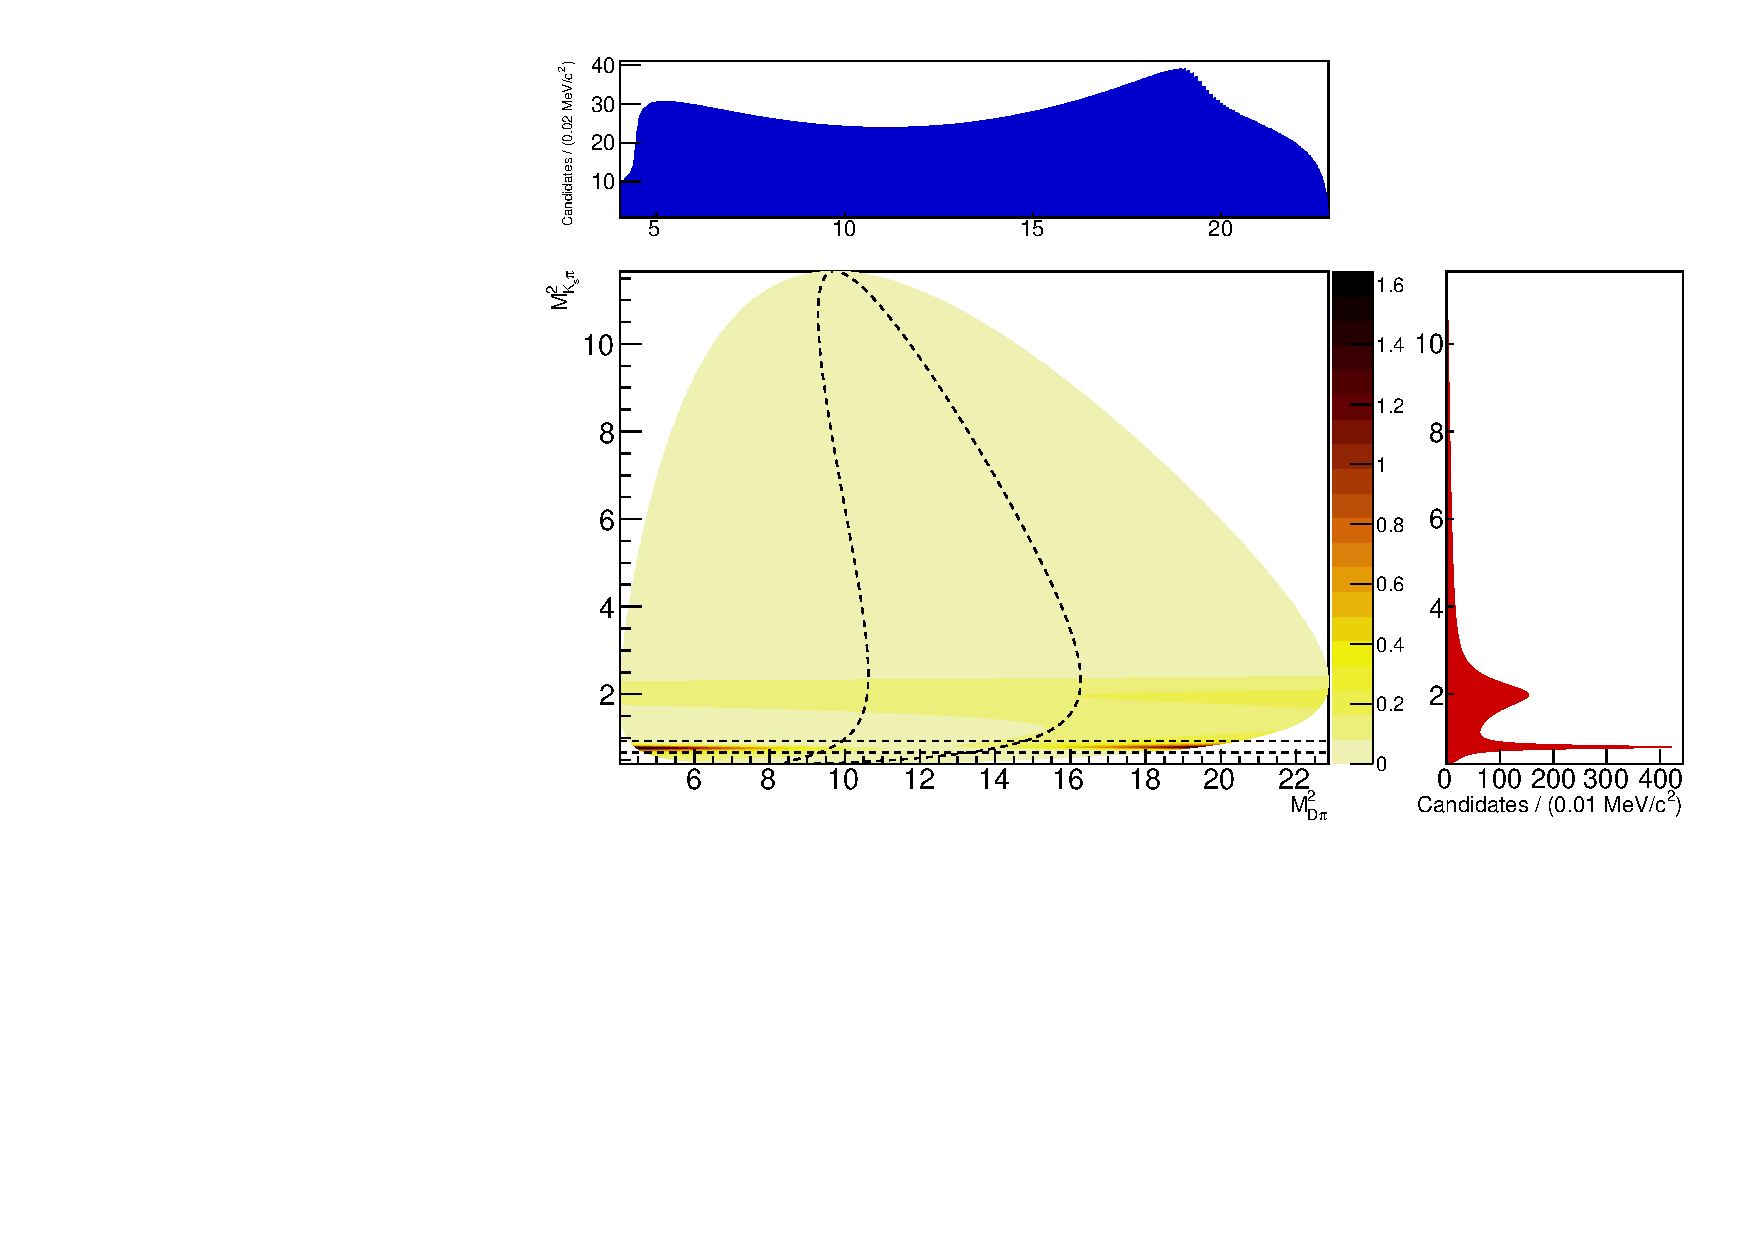
\includegraphics[width=0.8\linewidth]{figures/results/dalitz.pdf}
\caption{An example amplitude model used in the estimate of $\kappa$. The horizontal axis labelled $M_{D\pi}^2$ is defined as $(p_D + p_{\pi})^2$, where $p_{X}$ is the four-momentum of particle $X$. Similarly, the vertical axis, labelled $M_{K_s\pi}^2$, is defined as $(p_{K_s} + p_{\pi})^2$. The projections in these two coordinates are shown. The $K^*(892)^+$ and $K^*(1430)^+$ resonances can be clearly seen in the red projection on the right hand side of the figure. The dashed lines on the plot represent the \Kstar mass and \KS helicity angle selection used in this analysis.}
\label{dalitzplot}
\end{figure}

\subsection{Estimation of the coherence factor, $\kappa$}
\label{sec:interpretation:kappa}

One thousand variants of the amplitude model, described in Section \ref{sec:interpretation:model}, are generated, which differ in the amplitudes and phases of the components. These amplitudes and phases of the different resonances are varied within limits; the limits for the amplitudes are given in Section \ref{sec:interpretation:model} and all phases are generated randomly according to a flat distribution between $-\pi$ and $\pi$. The masses and widths of the resonances are kept constant at their central values, given in Table \ref{resonances}. 

For each model, $\kappa$ is computed, as the magnitude of the expression in Equation \ref{kappadefinition}, resulting in a distribution of $\kappa$ values estimated by the model, shown in Figure \ref{kappadistribution}. The mean and standard deviation of the resulting distribution provides an estimate of the central value and uncertainty of $\kappa$,  $0.95 \pm 0.04$. However, it is considered necessary to enhance the uncertainty of this estimate in order to account for the skewness of the distribution, therefore a final value of $\kappa = 0.95 \pm 0.06$ is used in this thesis to extract the physics parameters of interest.

\begin{figure}[h]
\centering
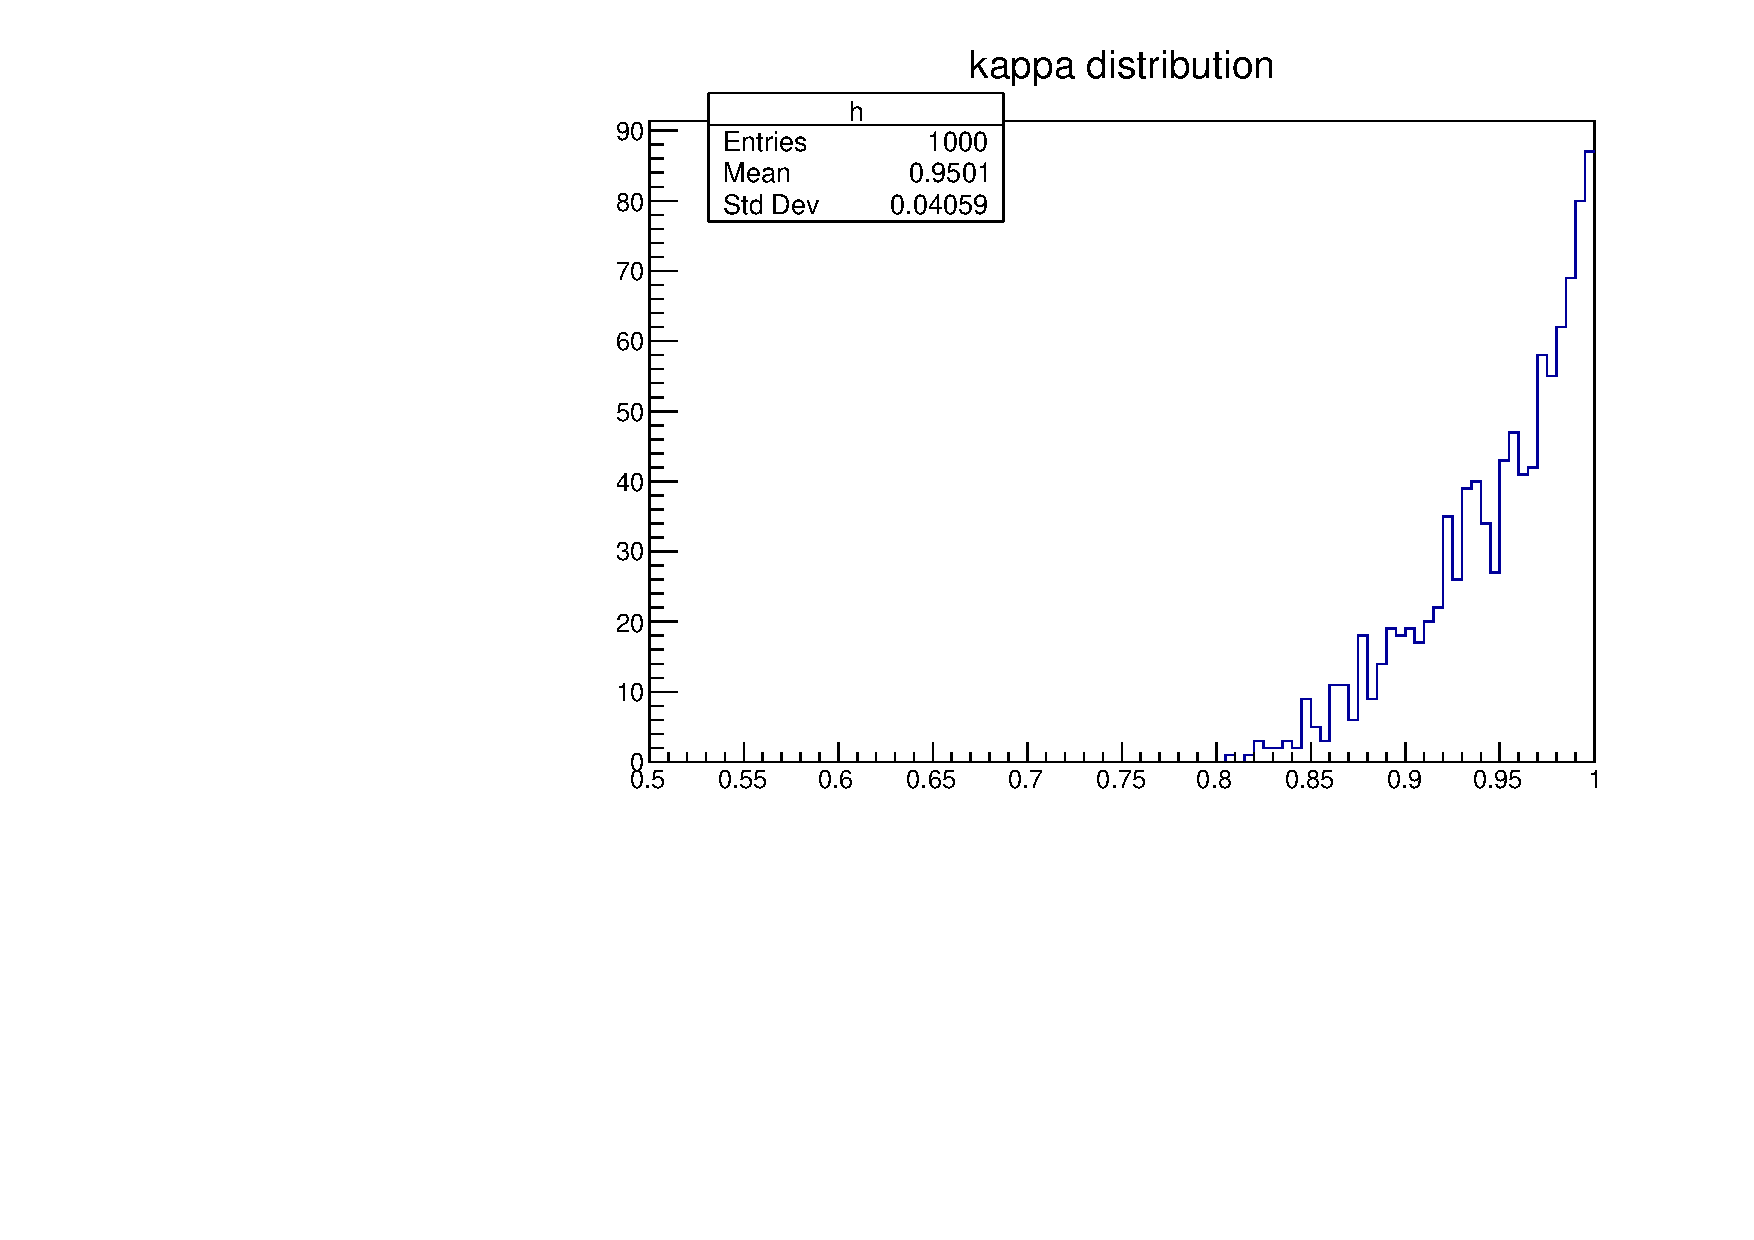
\includegraphics[trim = 0mm 0mm 0mm 8mm, clip, width=0.5\linewidth]{figures/results/kappa.pdf}
\caption{Distribution of the values of $\kappa$ from 1000 samples generated according the amplitude model.}
\label{kappadistribution}
\end{figure}

\section{Four-body phase space acceptance variations}
\label{sec:interpretation:inputs}

For multibody \decay{\Dz}{\Kmp\pipm\pimp\pipm} and \decay{\Dz}{\pip\pim\pip\pim} decays, some regions of phase space may exhibit larger \CP violation than other regions. In this analysis, an inclusive analysis over phase space is performed, therefore only the global \CP violation is considered, resulting in a loss of information. This loss of information gives rise to the four-body coherence factor, $R_{K3\pi}$, the integrated strong phase difference $\delta_D^{K3\pi}$ and the \CP-even fraction, $F_{4\pi}$.

The parameter $F_{4\pi}$ has been measured at CLEO-c, while the values for $\delta_D^{K3\pi}$ and $R_{K3\pi}$ are taken from combining \lhcb and CLEO-c results~\cite{charmk3pi,charmk3pi_errata,LHCb-PAPER-2015-057,charm4pi}. These measurements have been corrected for a flat efficiency. When making measurements at \lhcb, the \lhcb acceptance leads to small non-uniformities in efficiency, which could enhance or diminish asymmetry in certain regions of phase space. In order to use the measurements of $F_{4\pi}$, $\delta_D^{K3\pi}$ and $R_{K3\pi}$ in this analysis these effects must be assessed and accounted for by, either correcting for the \lhcb yields under a scenario of uniform efficiency, or adjusting the $F_{4\pi}$, $\delta_D^{K3\pi}$ and $R_{K3\pi}$ parameters to match the \lhcb efficiency variation. The efficiencies calculated in Section \ref{sec:cpfit:efficiencies} assumed an average efficiency across phase space. In order to correct for the \lhcb yields, eventwise efficiency corrections would have to be performed, which is not possible due to the large numbers of simulated events, and computing power, required. Therefore, the option of adjusting the $F_{4\pi}$, $\delta_D^{K3\pi}$ and $R_{K3\pi}$ parameters to match the \lhcb efficiency variation is preferred.

Figures \ref{dalitzk3pi} and \ref{dalitz4pi} show plots of projections of the four-body phase space distributions for \kpipipi and \pipipipi modes respectively. These plots are comparisons of distributions using simulated generator level signal events without any acceptance effects, and fully reconstructed simulated signal events used in this analysis. It can be seen that these distributions are very similar, suggesting that any differences due to \lhcb acceptance effects are very small, implying that $R_{K3\pi}$, $\delta_D^{K3\pi}$ and $F_{4\pi}$ can be used directly in the interpretation of \lhcb results.

\begin{figure}[h]
\centering
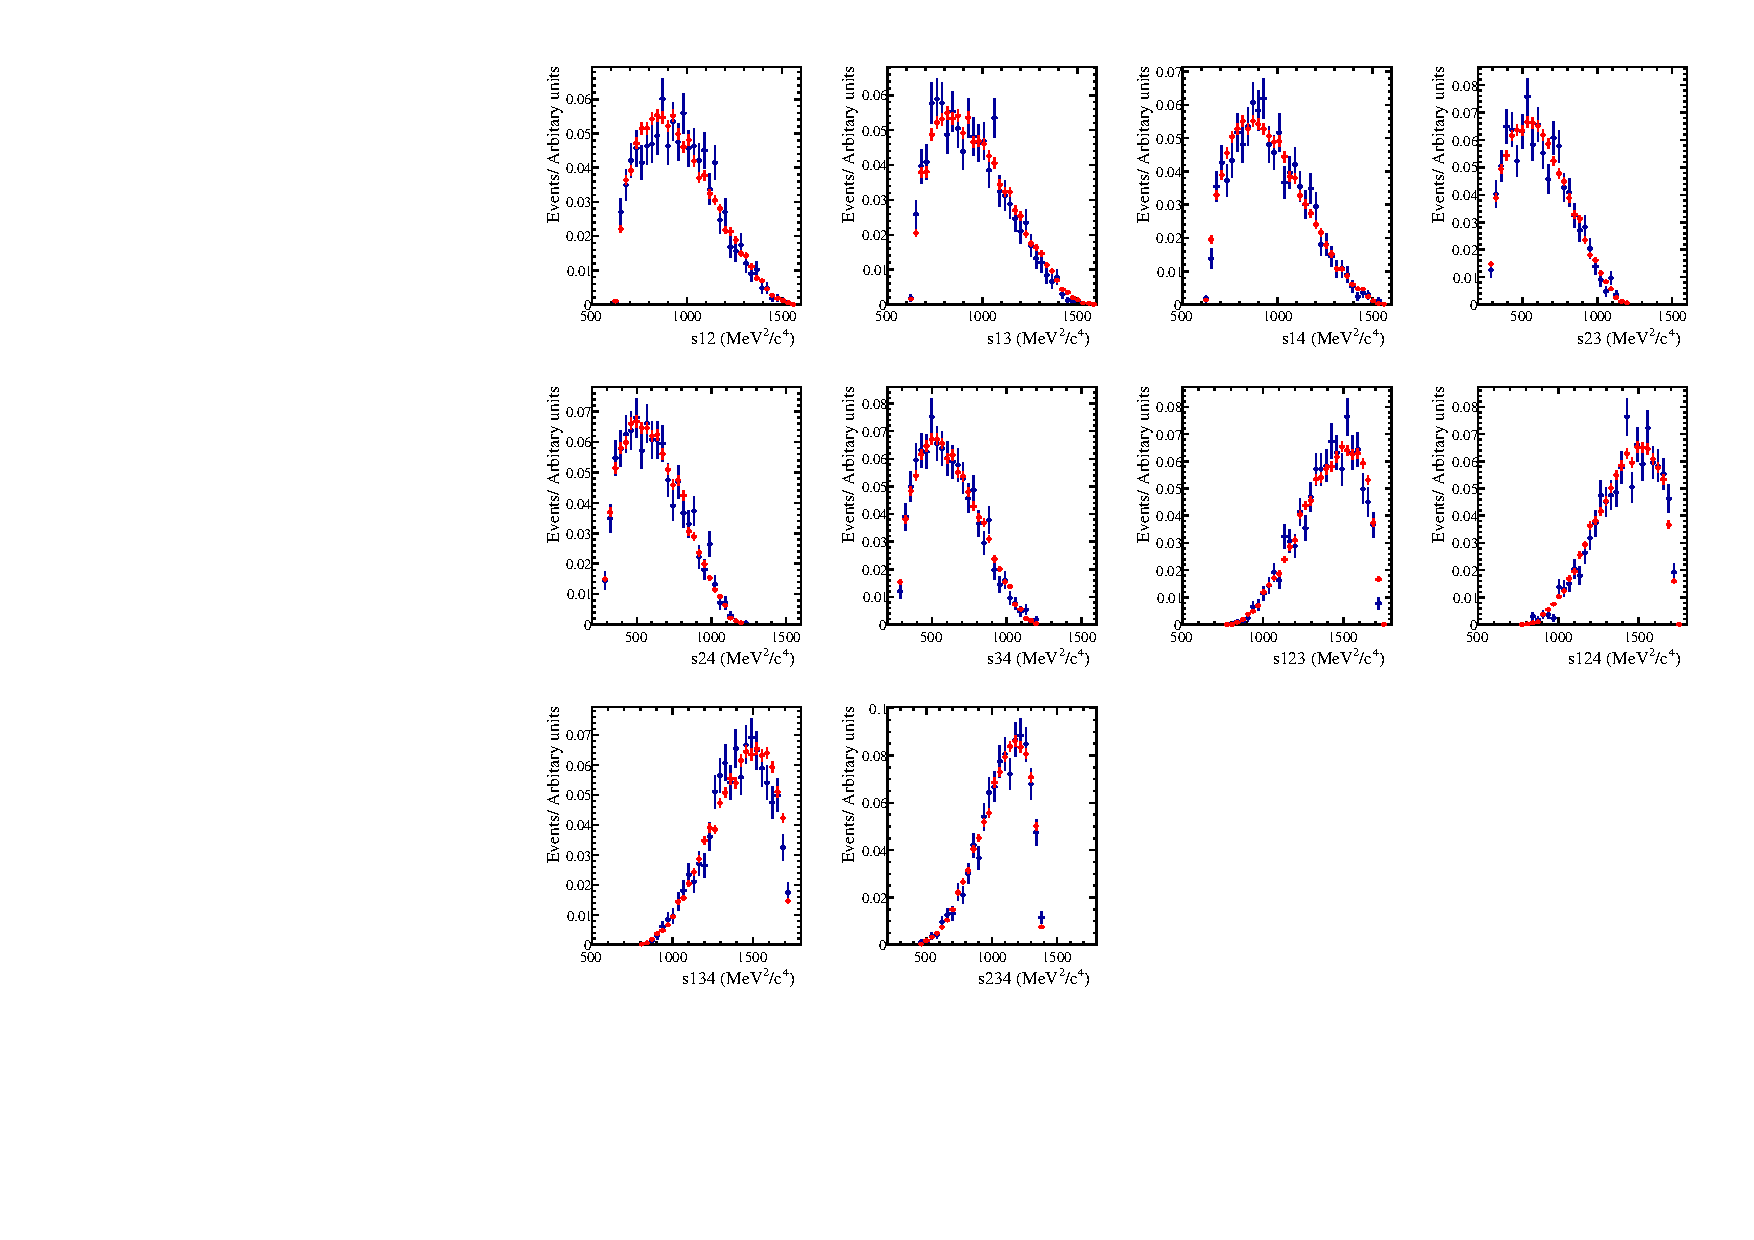
\includegraphics[width=0.9\linewidth]{figures/results/dalitzDist_KPiPiPi.pdf}
\caption{Distributions of invariant mass squared for all two- and three-particle \Dz daughter combinations with simulated generator level events (blue) and fully reconstructed and selected events (red) in the \kpipipi mode. The variable $sXY$ is defined as $(p_X + p_Y)^2$, where $X$ and $Y$ represent labels that refer to different \Dz daughters, and $p_X$ is the four-momentum of particle $X$. The different \Dz daughters labels are defined by: \decay{\Bm}{\D(K^-_1\pi^+_2\pi^-_3\pi^+_4)\Kstarm}.}
\label{dalitzk3pi}
\end{figure}

\begin{figure}[h]
\centering
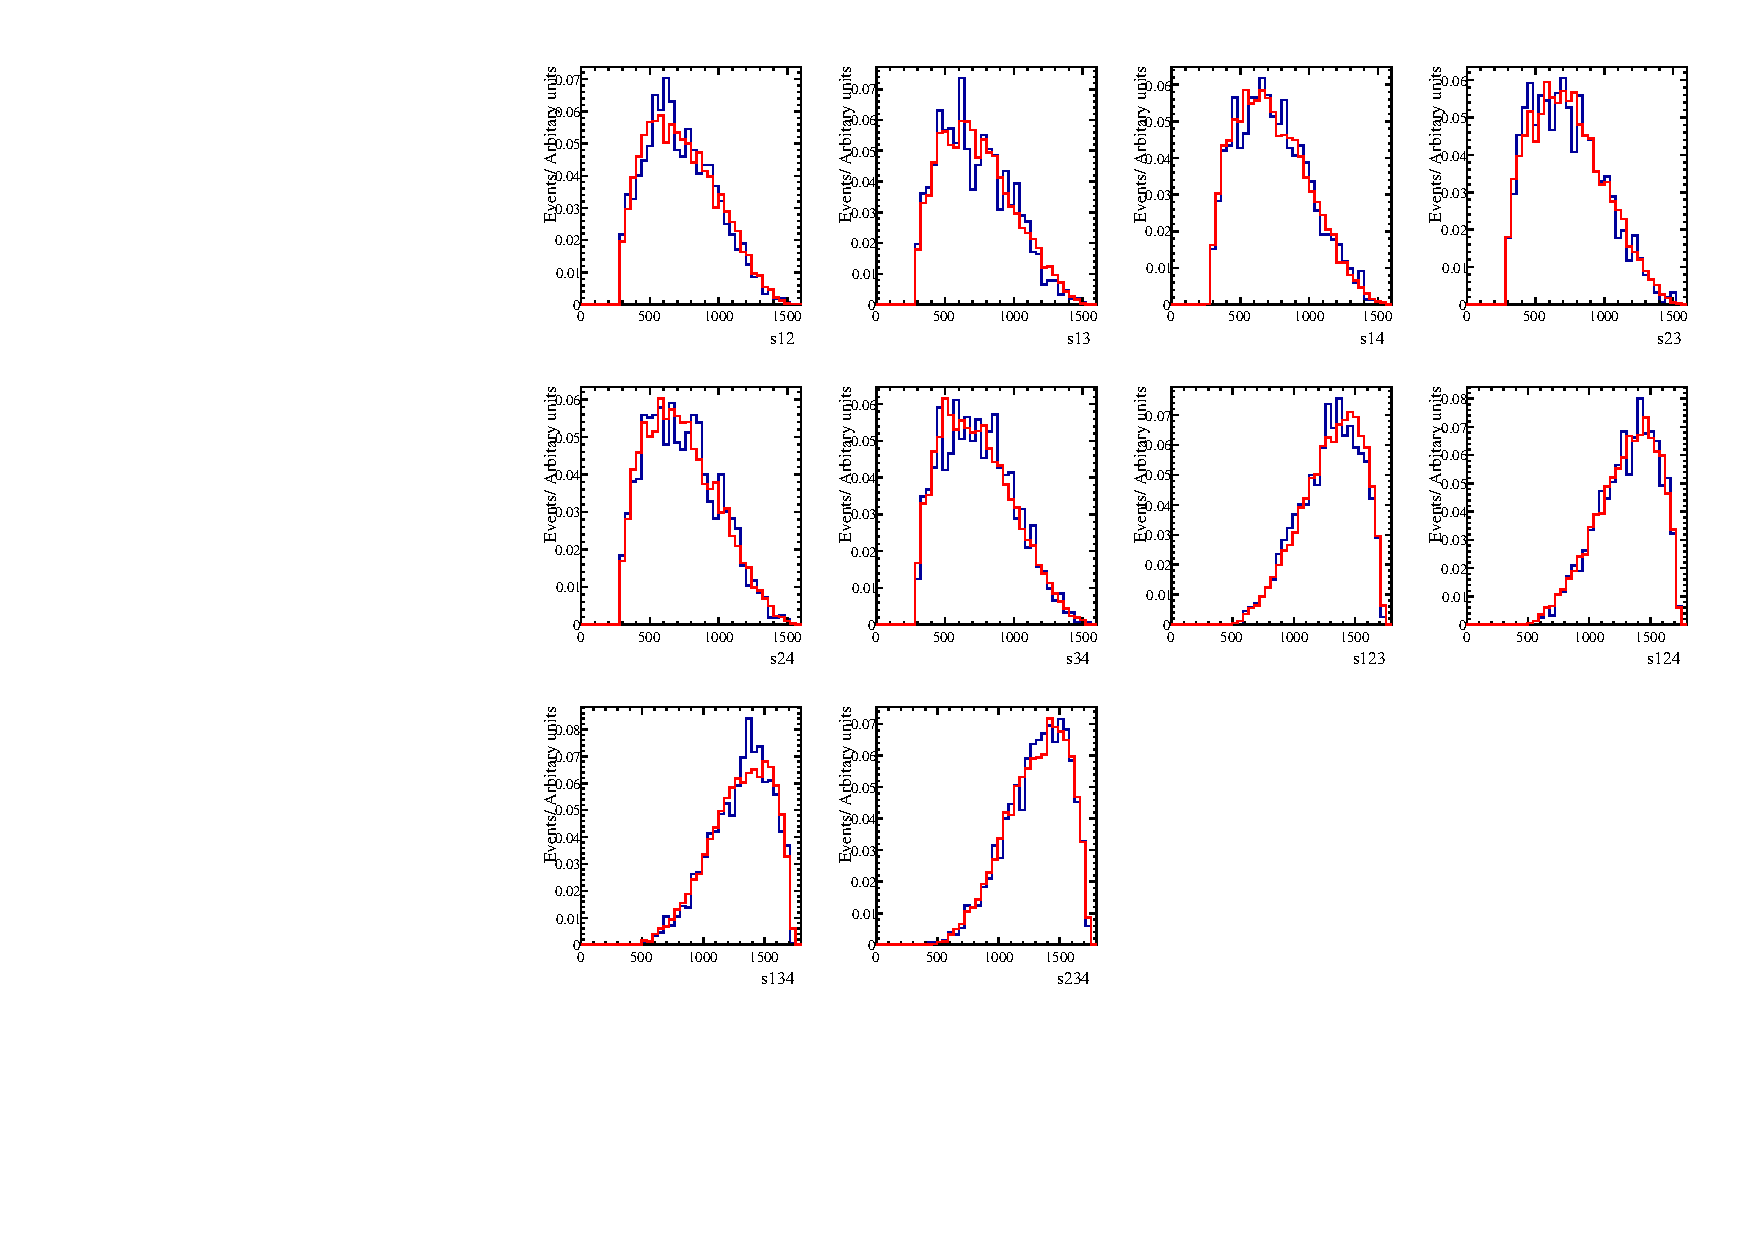
\includegraphics[width=0.9\linewidth]{figures/results/dalitzDist_PiPiPiPi.pdf}
\caption{Distributions of invariant mass squared for all two- and three-particle \Dz daughter combinations with simulated generator level events (blue) and fully reconstructed and selected events (red) in the \pipipipi mode. The variable $sXY$ is defined as $(p_X + p_Y)^2$, where $X$ and $Y$ represent labels that refer to different \Dz daughters, and $p_X$ is the four-momentum of particle $X$. The different \Dz daughters labels are defined by: \decay{\Bm}{\D(\pi^-_1\pi^+_2\pi^-_3\pi^+_4)\Kstarm}.}
\label{dalitz4pi}
\end{figure}

To verify this assumption, further studies are performed to assess whether the parameters $R_{K3\pi}$ and $\delta_D^{K3\pi}$ require any corrections, when used in this thesis. To assess the effects of small variation in the four-body phase space for \kpipipi decays, the coherence factor and strong phase are calculated from a preliminary version of the \decay{\Dz}{\Km\pip\pim\pip} amplitude model described in Ref.~\cite{LHCb-PAPER-2017-040}, both under the assumption of uniform acceptance and total \lhcb acceptance. The differences between these two scenarios gives an estimate of the corrections that should be applied to the $R_{K3\pi}$ and $\delta_D^{K3\pi}$ before being used in the \lhcb interpretation. The difference is calculated to be 0.002 for the coherence factor and 0.7$^{\circ}$ for the strong phase difference. The values of the inputs are $R_{K3\pi} = 0.43^{+0.17}_{-0.13}$ and $\delta_D^{K3\pi} = \left(128^{+28}_{-17}\right)$, taken from a combination of CLEO-c and \lhcb results~\cite{charmk3pi,charmk3pi_errata,LHCb-PAPER-2015-057}. Therefore, the size of the corrections due to the \lhcb phase space acceptance are negligible in comparison to the CLEO-c/LHCb uncertainties and hence no further action is taken. This study was possible as the \decay{\Dz}{\Km\pip\pim\pip} amplitude model was already being developed for a different purpose.

The distributions in Figure \ref{dalitz4pi} are shown to be very similar, which suggests that the fractional \CP content, $F_{4\pi}$, from CLEO-c can be used directly in the interpretation of \lhcb results. Therefore, the value of $F_{4\pi}$ is taken directly from the CLEO-c measurement, $0.734 \pm 0.028$~\cite{charm4pi}. While a similar study, as described for \decay{\Dz}{\Km\pip\pim\pip}, could have been carried out, a model was not available at the time~\footnote{Although a \decay{\Dz}{\pim\pip\pim\pip} amplitude model has subsequently been published~\cite{4piamplitude}}. Therefore more detailed quantitative studies into the effect of any differences in acceptance on the value of $F_{4\pi}$ are not performed. As the correction on the $R_{K3\pi}$ and $\delta_D^{K3\pi}$ values due to the \lhcb acceptance has been shown to be almost two orders of magntiude smaller than the measured uncertainties, it can reasonably assumed that the coressponding effect on the $F_{4\pi}$ result is also negligible. Therefore, it is concluded that small variations in efficiency lead to a negligible correction in the observables. 


\section{Results in terms of $r_B$, $\delta_B$ and \Pgamma}
\label{sec:interpretation:gammadini}

The \CP observables and other parameters, namely $\kappa$, $r_D^{K\pi}$, $\delta_D^{K\pi}$, $r_D^{K3\pi}$, $\delta_D^{K3\pi}$, $R_{K3\pi}$ and $F_{4\pi}$, are combined. Constraining these parameters, as opposed to using them as fixed inputs, allows the possibility of the \CP observables providing additional sensitivity to these parameters. While the dataset here is too small to have an impact, it is common in the presentation of \lhcb results to constrain these parameters to the values given in Table \ref{inputparameters}. A global $\chi^2$ minimisation is performed, taking correlations into account, where
\begin{equation}
\chi^2 = (x(\theta) - x_0)^TV_0^{-1}(x(\theta)-x_0) \text{ . }
\end{equation}
In this expression, $x(\theta)$ is the set of observables calculated from the fundamental set of physics parameters, $\theta$, as well as the parameters, $\kappa$, $r_D^{K\pi}$, $\delta_D^{K\pi}$, $r_D^{K3\pi}$, $\delta_D^{K3\pi}$, $R_{K3\pi}$ and $F_{4\pi}$. The set, $x_0$, are the measured values of the observables and parameters, and $V_0$ is the covariance matrix. The sensitivity of a given parameter is determined by calculating the $\chi^2$ at fixed points in parameter space. The difference between this calculated $\chi^2$ value and that of the global minimum, $\Delta\chi^2$, quantifies the confidence in the global minimum. The $\chi^2$ value at the global minimum is 3.0 with 9 degrees of freedom. The confidence level for any pair of parameters is calculated assuming that these are normally distributed, which enables the $\Delta \chi^2 = 2.30,\ 6.18,\ 11.8$ contours to be drawn, corresponding to 68.3\%, 95.5\%, 99.7\% confidence levels, respectively. 

\begin{table}
\centering
\begin{tabular}{cc}
Fit parameter & Value \\
\hline
$\kappa$ & $0.96 \pm 0.06$ \\
$r_D^{K\pi}$ & $0.0591 \pm 0.0003$ \\
$\delta_D^{K\pi}$ & $191.8 \pm 12.1$ \\
$r_D^{K3\pi}$ & $0.0549 \pm 0.0006$ \\
$\delta_D^{K3\pi}$ & $128 \pm 28$ \\
$R_{K3\pi}$ & $0.43 \pm 0.17$ \\
$F_{4\pi}$ & $0.737 \pm 0.028$
\end{tabular}
\caption{Values of the external inputs used as constraints. These values are taken from Ref.~\cite{HFAG,charmk3pi,charmk3pi_errata,LHCb-PAPER-2015-057,charm4pi}.}
\label{inputparameters}
\end{table}

Figures \ref{gammadiniplots2body} and \ref{gammadiniplotsallmodes} give 2D contour plots of $r_B$ versus \Pgamma and $\delta_B$ versus \Pgamma. Figure \ref{gammadiniplots2body} shows the contour plots using the \CP observables from the two-body modes only and Figure \ref{gammadiniplotsallmodes} show the contour plots using the \CP observables from both the two- and four-body decays. The addition of the four-body modes improves the constraints on the physics parameters and provides additional distinction between the two minima. 

The data are consistent with the value of $\gamma$ indicated by previous measurements~\cite{LHCb-PAPER-2016-032, CKMFitter}, $\sim 70^\circ$. The values of $r_B$, $\delta_B$ and \Pgamma are determined at the point where the global $\chi^2$ of the fit is minimised. The value of \rb is calculated to be $r_B = 0.113^{+0.015}_{-0.021}$. The parameter \deltab has a measured central value of $43.0^{\circ}$ with a $1\sigma$ confidence interval of $[25.9, 61.9]^{\circ}$, and $2\sigma$ confidence intervals of $[8.2, 83.9]^{\circ}$ and $[100.7,175.8]^{\circ}$. The central value of \Pgamma is measured to be $40.9^{\circ}$ with a $1\sigma$ confidence interval of $[24.7, 60.2]^{\circ}$, and $2\sigma$ confidence intervals of $[10.2, 86.1]^{\circ}$ and $[100.0,165.2]^{\circ}$. No value of \Pgamma or \deltab is excluded at the $3\sigma$ level. These results provide the current best sensitivity to the hadronic parameters of the \Bm decay, \rb and \deltab.

\begin{figure}[h]
\centering
\subfloat[$r_B$ versus \Pgamma]{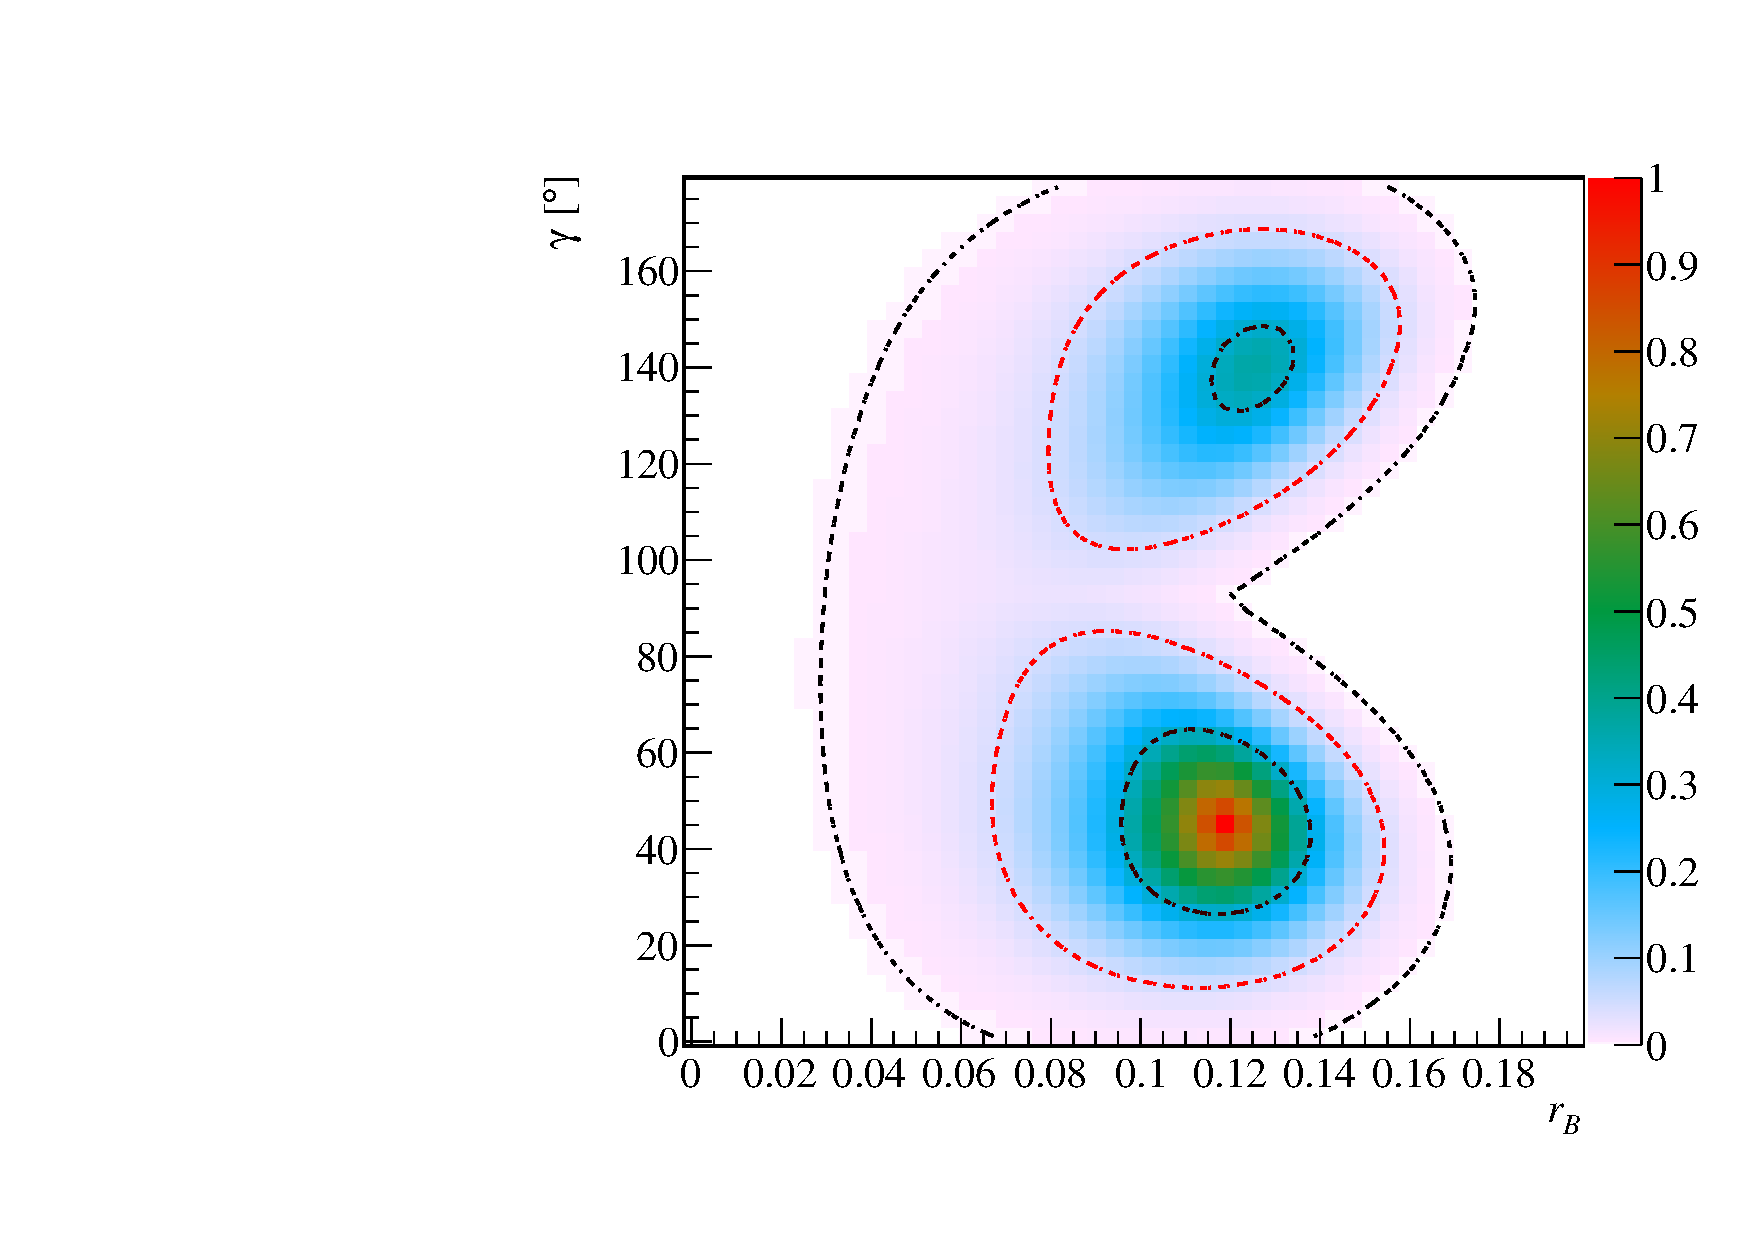
\includegraphics[width=0.5\linewidth]{figures/interpretation/rBu_dkstar_gamma_2Dscan_nomixing_2body.pdf}}
\subfloat[$\delta_B$ versus \Pgamma]{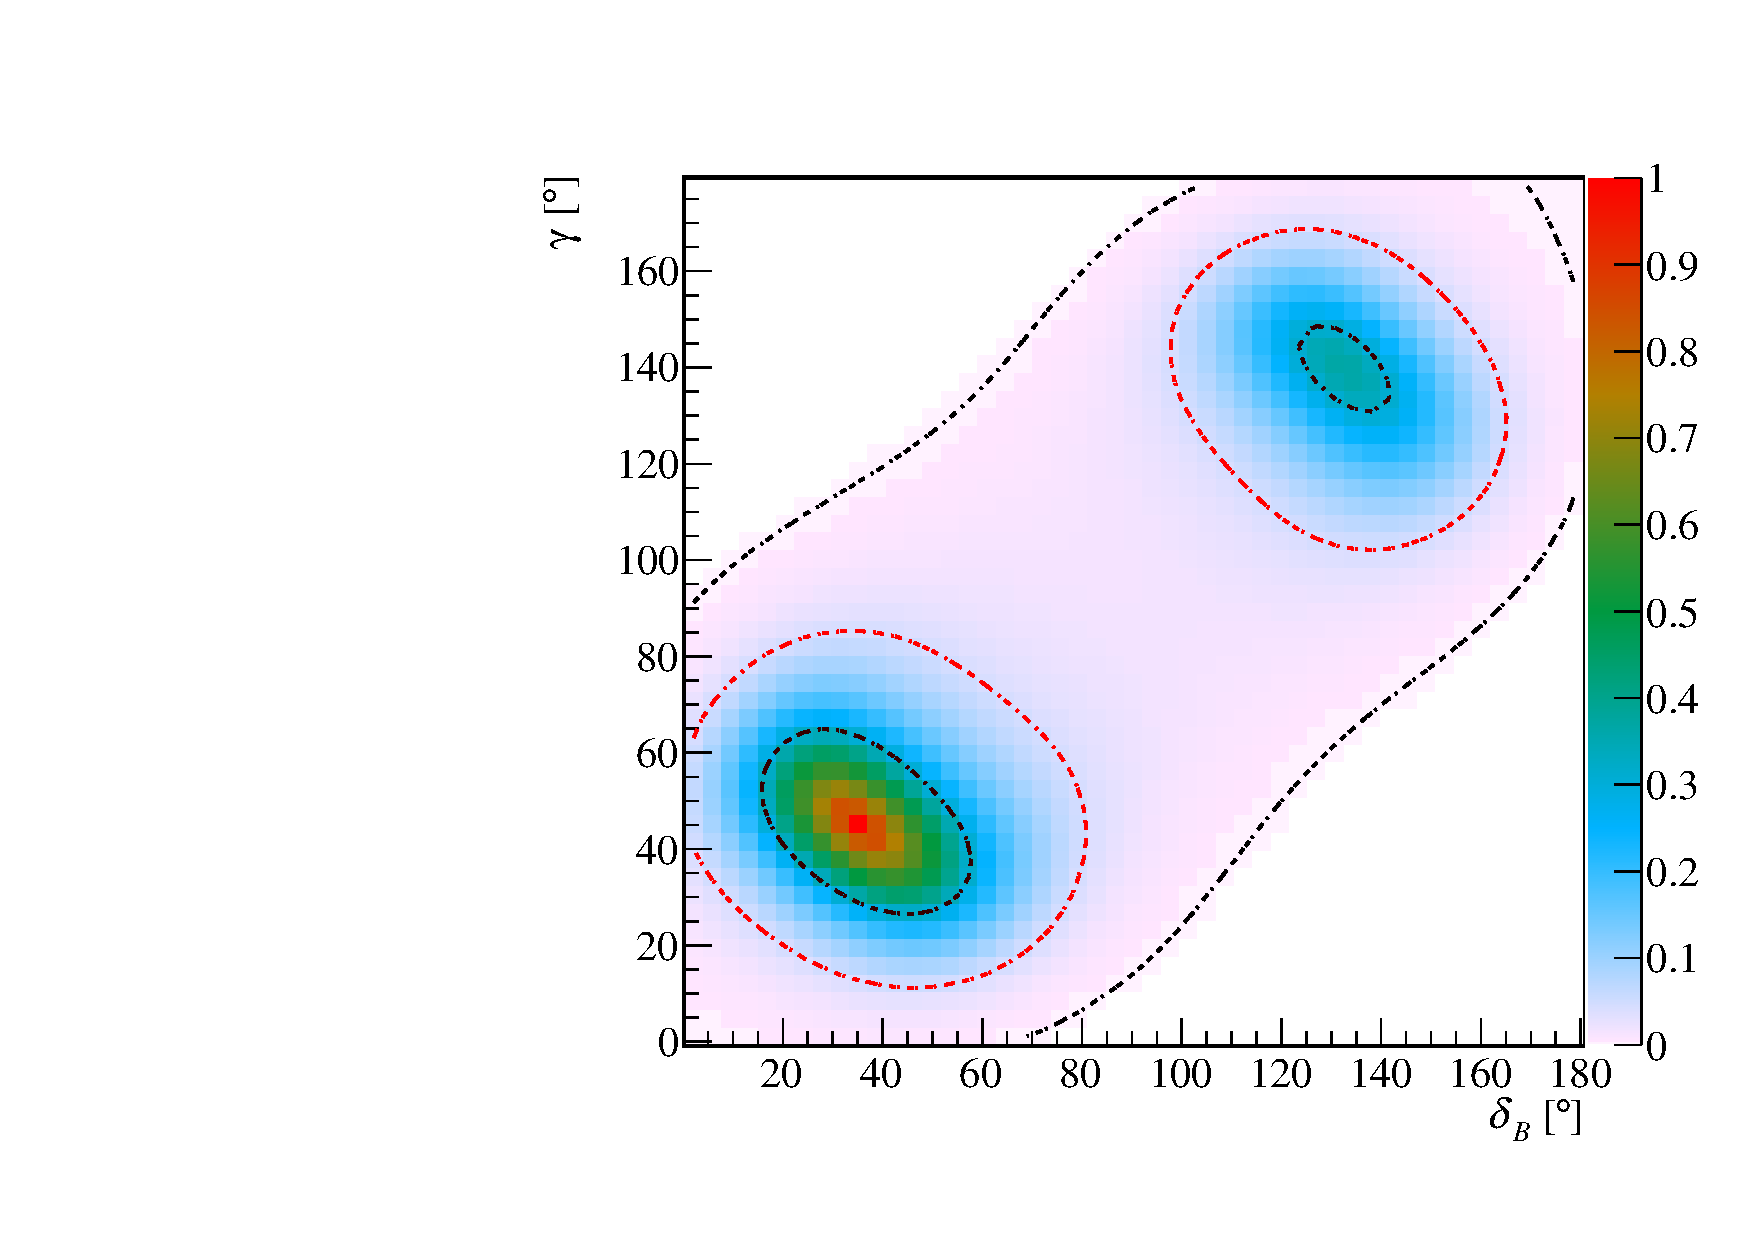
\includegraphics[width=0.5\linewidth]{figures/interpretation/deltaBu_dkstar_gamma_2Dscan_nomixing_2body.pdf}}
\caption{Contour plots showing 2D scans of the physics parameters using the two-body modes only. The dashed lines represent the $\Delta \chi^2 = 2.30,\ 6.18,\ 11.8$ contours, corresponding to 68.3\%, 95.5\%, 99.7\% confidence levels (CL), respectively. The colour scale represents 1 - CL.}
\label{gammadiniplots2body}
\end{figure}

\begin{figure}[h]
\centering
\subfloat[$r_B$ versus \Pgamma]{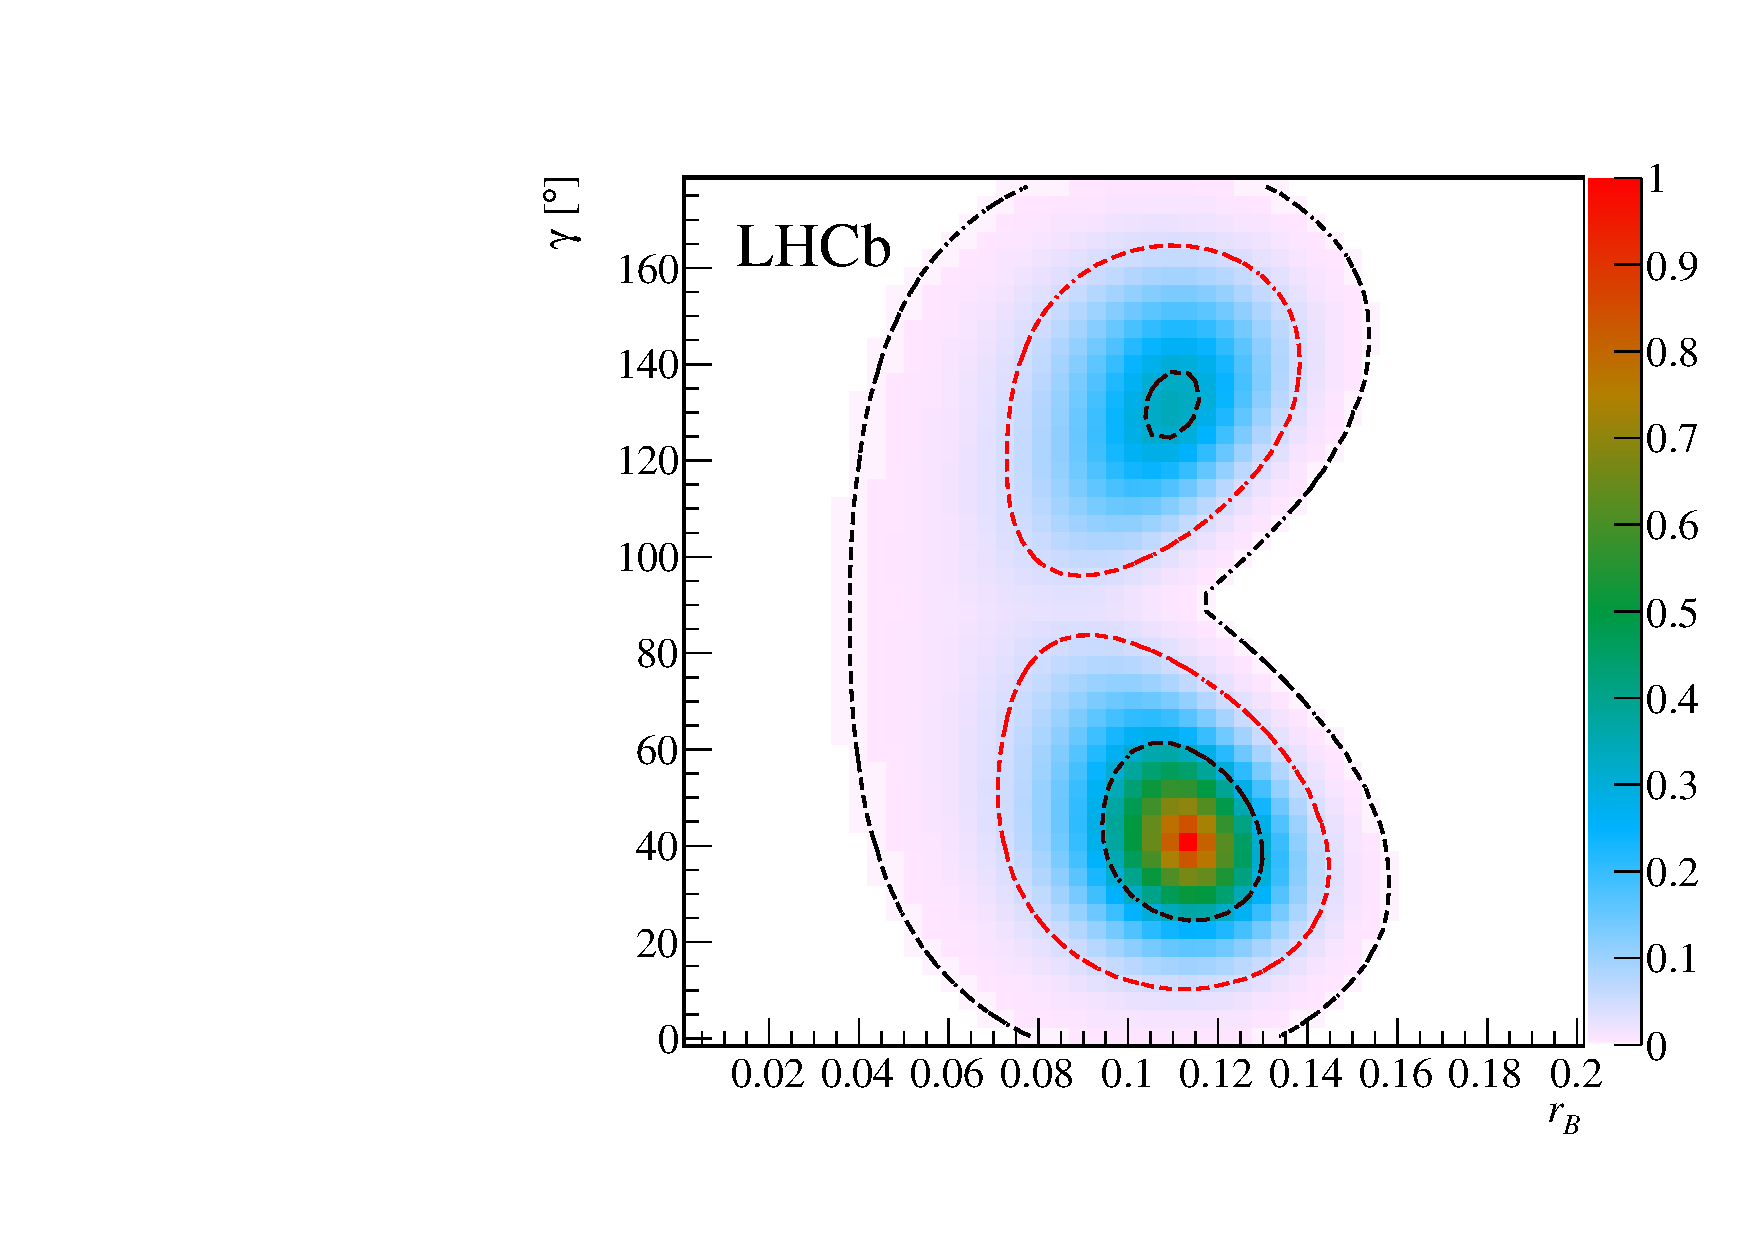
\includegraphics[width=0.5\linewidth]{figures/interpretation/rBu_dkstar_gamma_2Dscan_nomixing_all.pdf}}
\subfloat[$\delta_B$ versus \Pgamma]{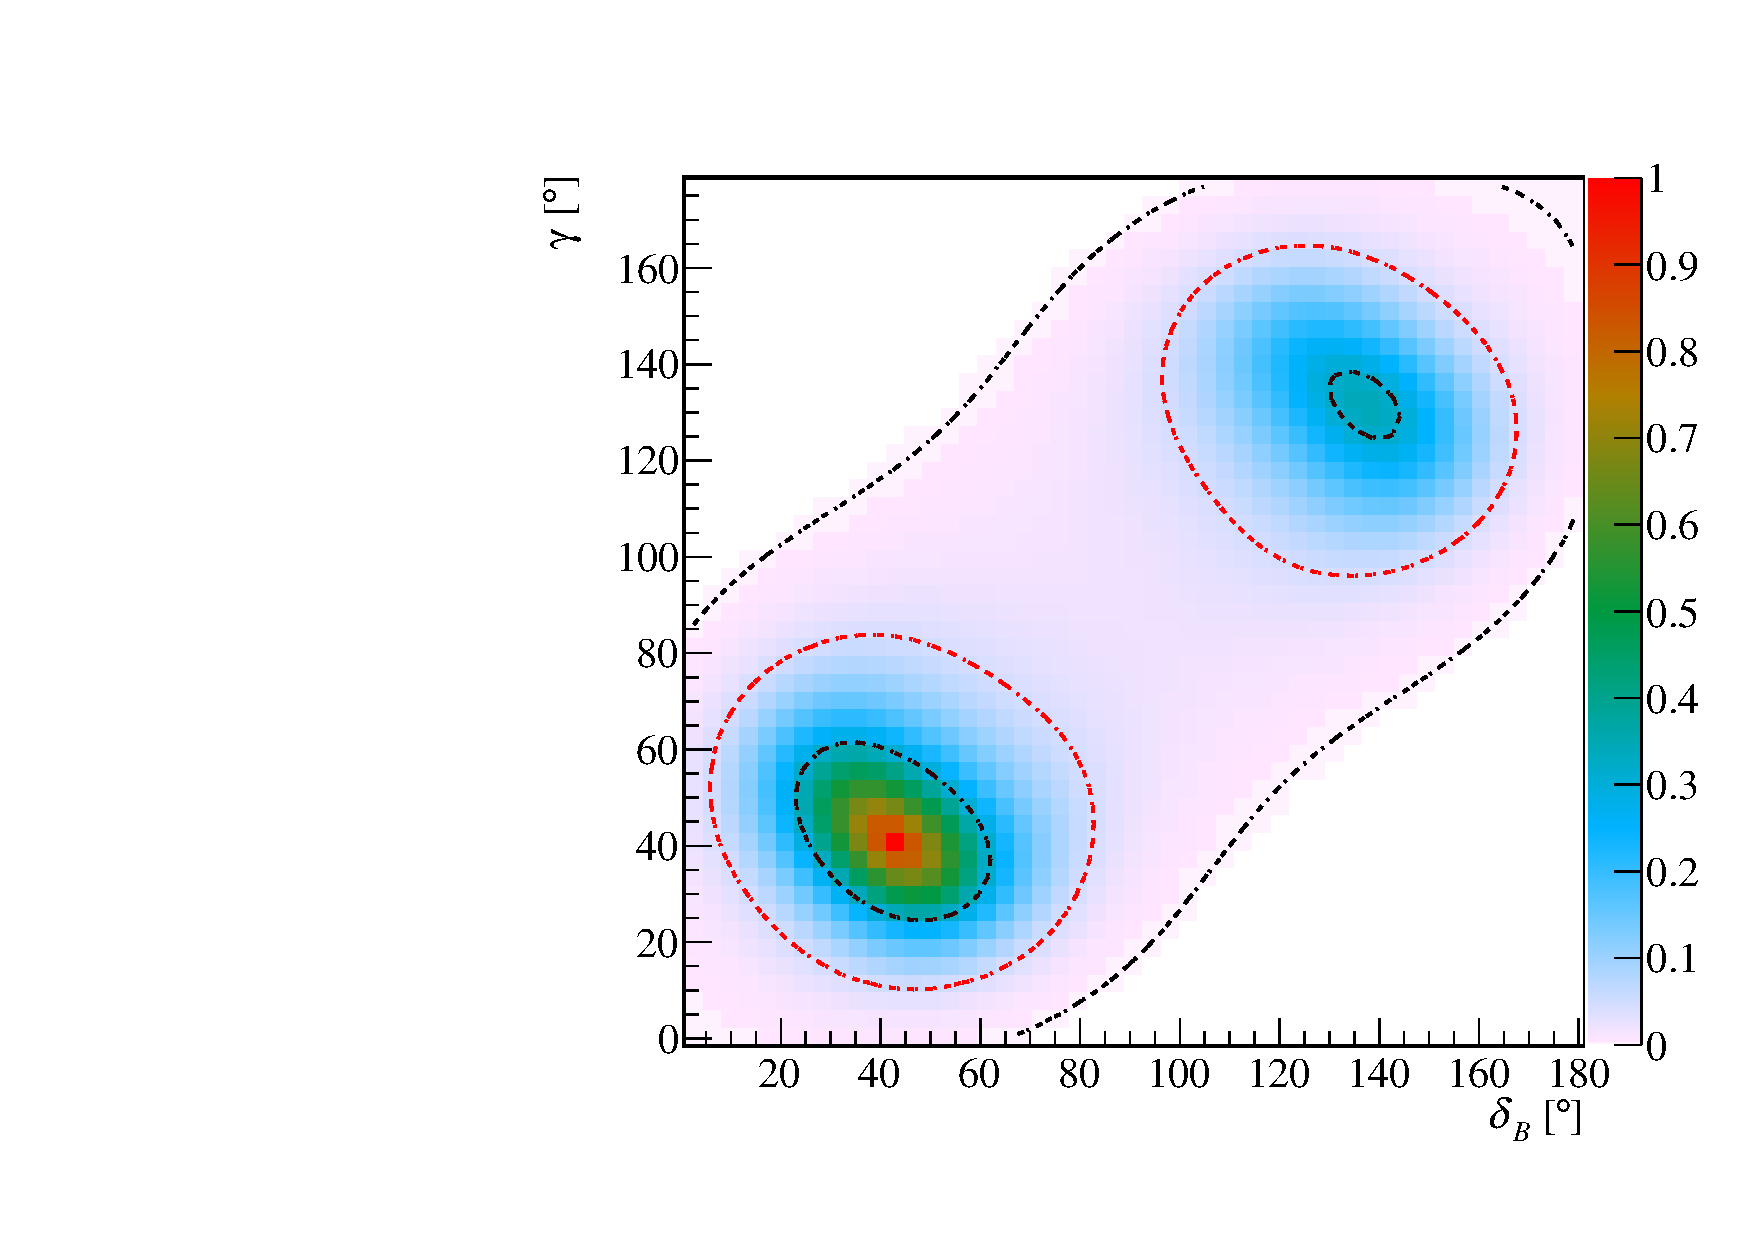
\includegraphics[width=0.5\linewidth]{figures/interpretation/deltaBu_dkstar_gamma_2Dscan_nomixing_all.pdf}}
\caption{Contour plots showing 2D scans of the physics parameters using both the two- and four-body modes. The dashed lines represent the $\Delta \chi^2 = 2.30,\ 6.18,\ 11.8$ contours, corresponding to 68.3\%, 95.5\%, 99.7\% confidence levels (CL), respectively. The colour scale represents 1 - CL.}
\label{gammadiniplotsallmodes}
\end{figure}

\section{Expected future sensitivity to $r_B$, $\delta_B$ and \Pgamma}
\label{sec:interpretation:futuresensitivity}

In this thesis, the \btodkst mode has shown an increase of three times the yield per unit integrated luminosity from \runone to \runtwo, mainly due to the increase in centre of mass energy of the $pp$ collisions from 7 and 8\tev to 13\tev. As previously stated, the data used in this analysis was collected in 2011 and 2012, forming the \runone \dataset, and 2015 and 2016, forming part of the \runtwo \dataset. The current running period of the LHC, namely \runtwo, is currently ongoing until the end of 2018, and Run 3 is the next running period, planned to take place between 2021 and 2023.

The projected yields for the end of Run 2 and the end of Run 3 are estimated using the forecasts for the stored integrated luminosity and expected improvements in detector performance during these data-taking periods. The projections of the integrated luminosities can be found in \tab~\ref{projectedyields}. It is assumed that the yield per unit integrated luminosity remains the same for the rest of \runtwo, which is a reasonable assumption as there are no expected significant changes to the detector or running conditions. Between Run 2 and Run 3 the detector will undergo an upgrade to improve detector performance. Improvements to the detector, trigger and reconstruction will be made, including moving to a fully software-based trigger~\cite{CERN-LHCC-2014-016} and the rebuilding of many detector components. These improvements to the detector will allow the experiment to run at an instantaneous luminosity of $2 \times 10^{33} cm^{-2}s^{-1}$, five times larger than the current conditions~\cite{CERN-LHCC-2014-016}. Therefore, Run 3 is expected to produce a minimum of 5\invfb per year for three years~\cite{CERN-LHCC-2014-016}. The upgrade to a fully software-based trigger improves the trigger efficiencies for the fully hadronic modes by about a factor of two compared to \runone~\cite{CERN-LHCC-2014-016}. Additionally, the centre of mass energy is expected to increase to 14\tev. Based on the observed improvement in \runtwo due to the increased centre of mass energy, and the expected improvements in Run 3 from the upgrade of the detector, yields of \B meson decay modes in Run 3 are expected to increase by a factor of $\sim$32 compared to \runone, assuming no improvements in the analysis procedure. The result of these assumptions are shown in the projected estimates in Table~\ref{projectedyields}.

\begin{table}
\resizebox{\textwidth}{!}{
\begin{tabular}{cccc}
\hline
Year & Integrated Luminosity & \kpi yield & Yield per \invfb \\
\hline
\runone & 3\invfb & 725 & 242 \\
\runtwo (up to 2016) & 1.8\invfb & 1390 & 771 \\
\textbf{Run 2 (after 2016)} & \textbf{3.2\invfb} & \textbf{2466} & \textbf{771} \\
\textbf{Run 3} & \textbf{15\invfb} & \textbf{23130} & \textbf{1542} \\
\hline
\end{tabular}}
\caption{Yields and projected yields for different data-taking periods of the LHC. The entries in bold are projected yields, whereas the other entries refer to data used in this thesis. Projected results are justified in the text, with information taken from Ref.~\cite{CERN-LHCC-2014-016}.}
\label{projectedyields}
\end{table}

% Luminosity/Yield factor for Run 2: 2.2
% Luminosity/Yield factor for Run 3: 13.1

Using the results from \tab~\ref{projectedyields}, the projected future sensitivity to the physics parameters \rb, \deltab and \Pgamma are estimated, assuming that the systematic uncertainties remain the same. Figure \ref{gammadiniplotsrun2} gives the projected results at the end of Run 2 as 2D contour plots of \rb versus \Pgamma and \deltab versus \Pgamma. The equivalent plots for the end of Run 3 are shown in Figure \ref{gammadiniplotsrun3}. 

\begin{figure}[h]
\centering
\subfloat[\rb versus \Pgamma]{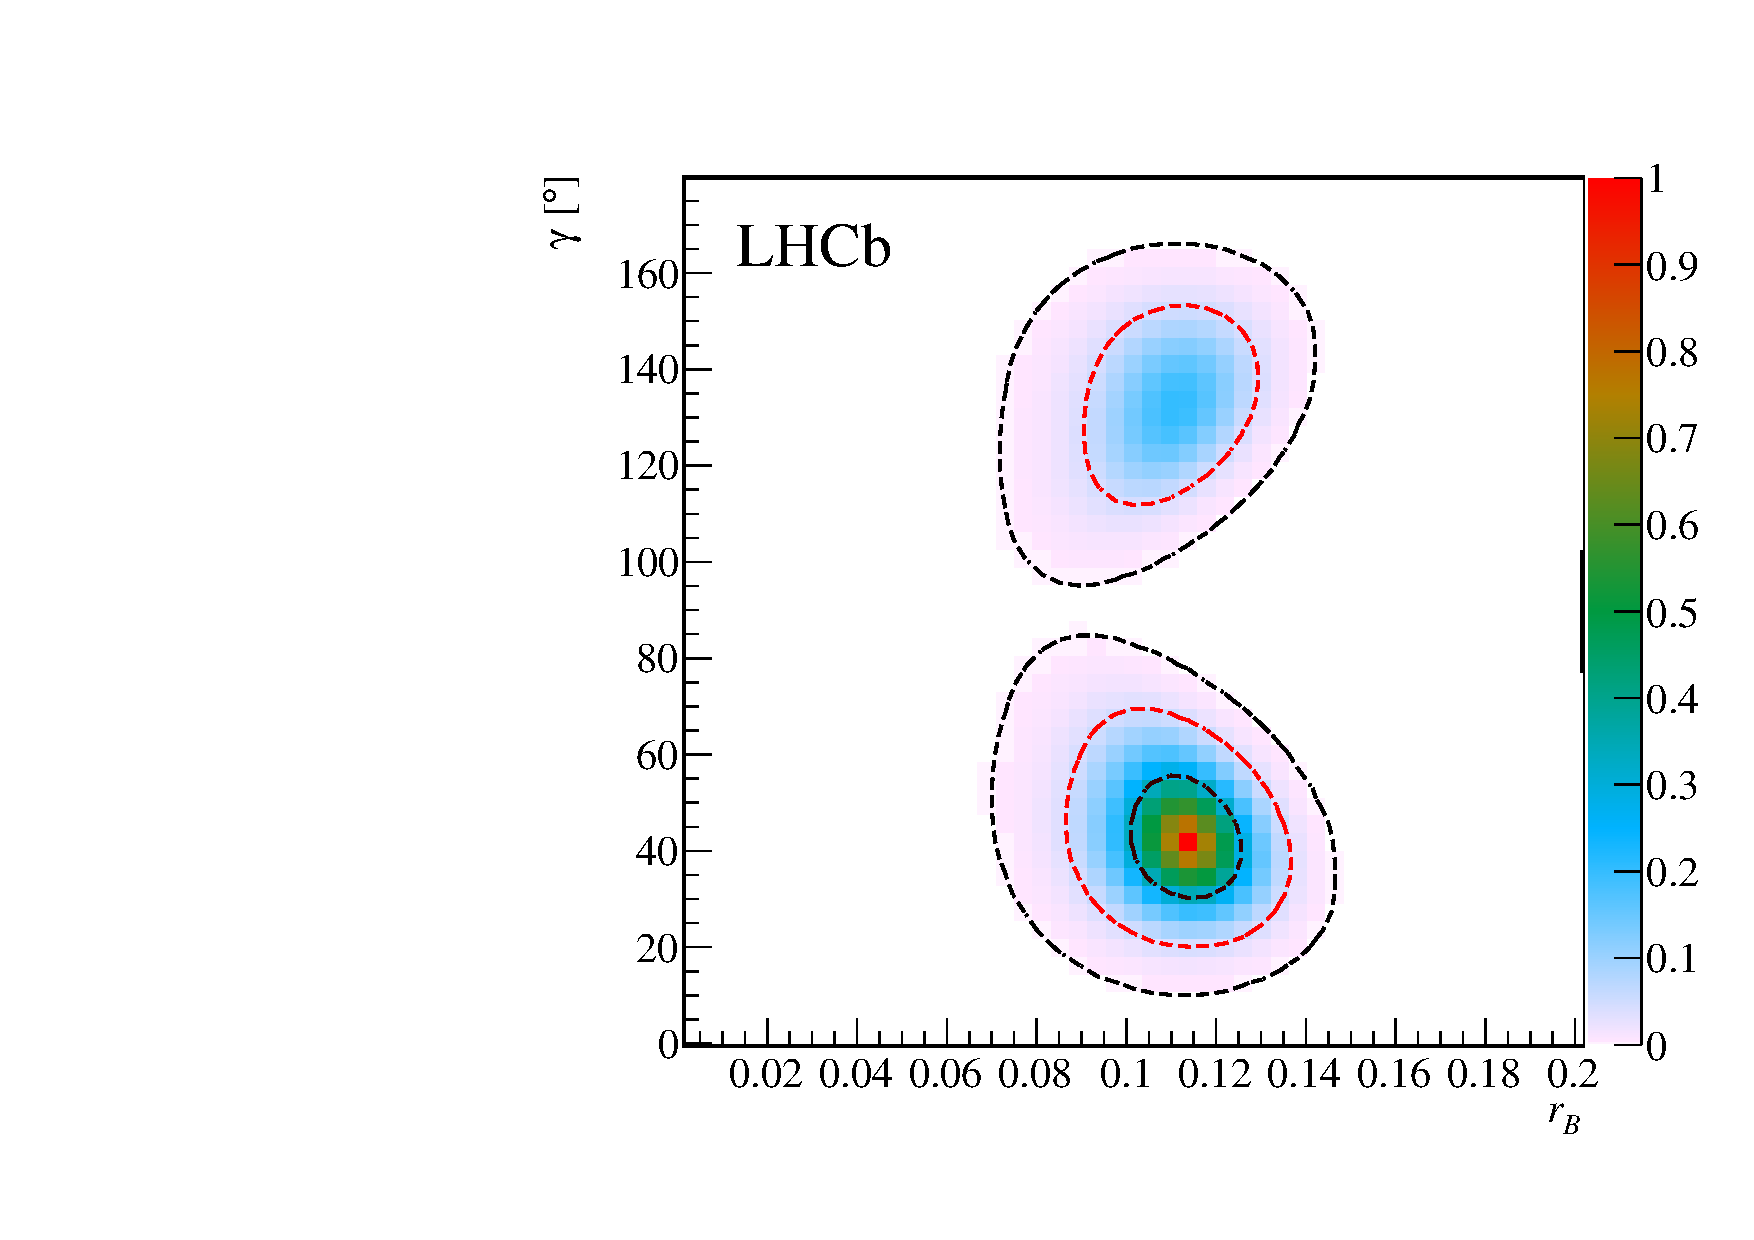
\includegraphics[width=0.5\linewidth]{figures/interpretation/rBu_dkstar_gamma_2Dscan_nomixing_Run2.pdf}}
\subfloat[\deltab versus \Pgamma]{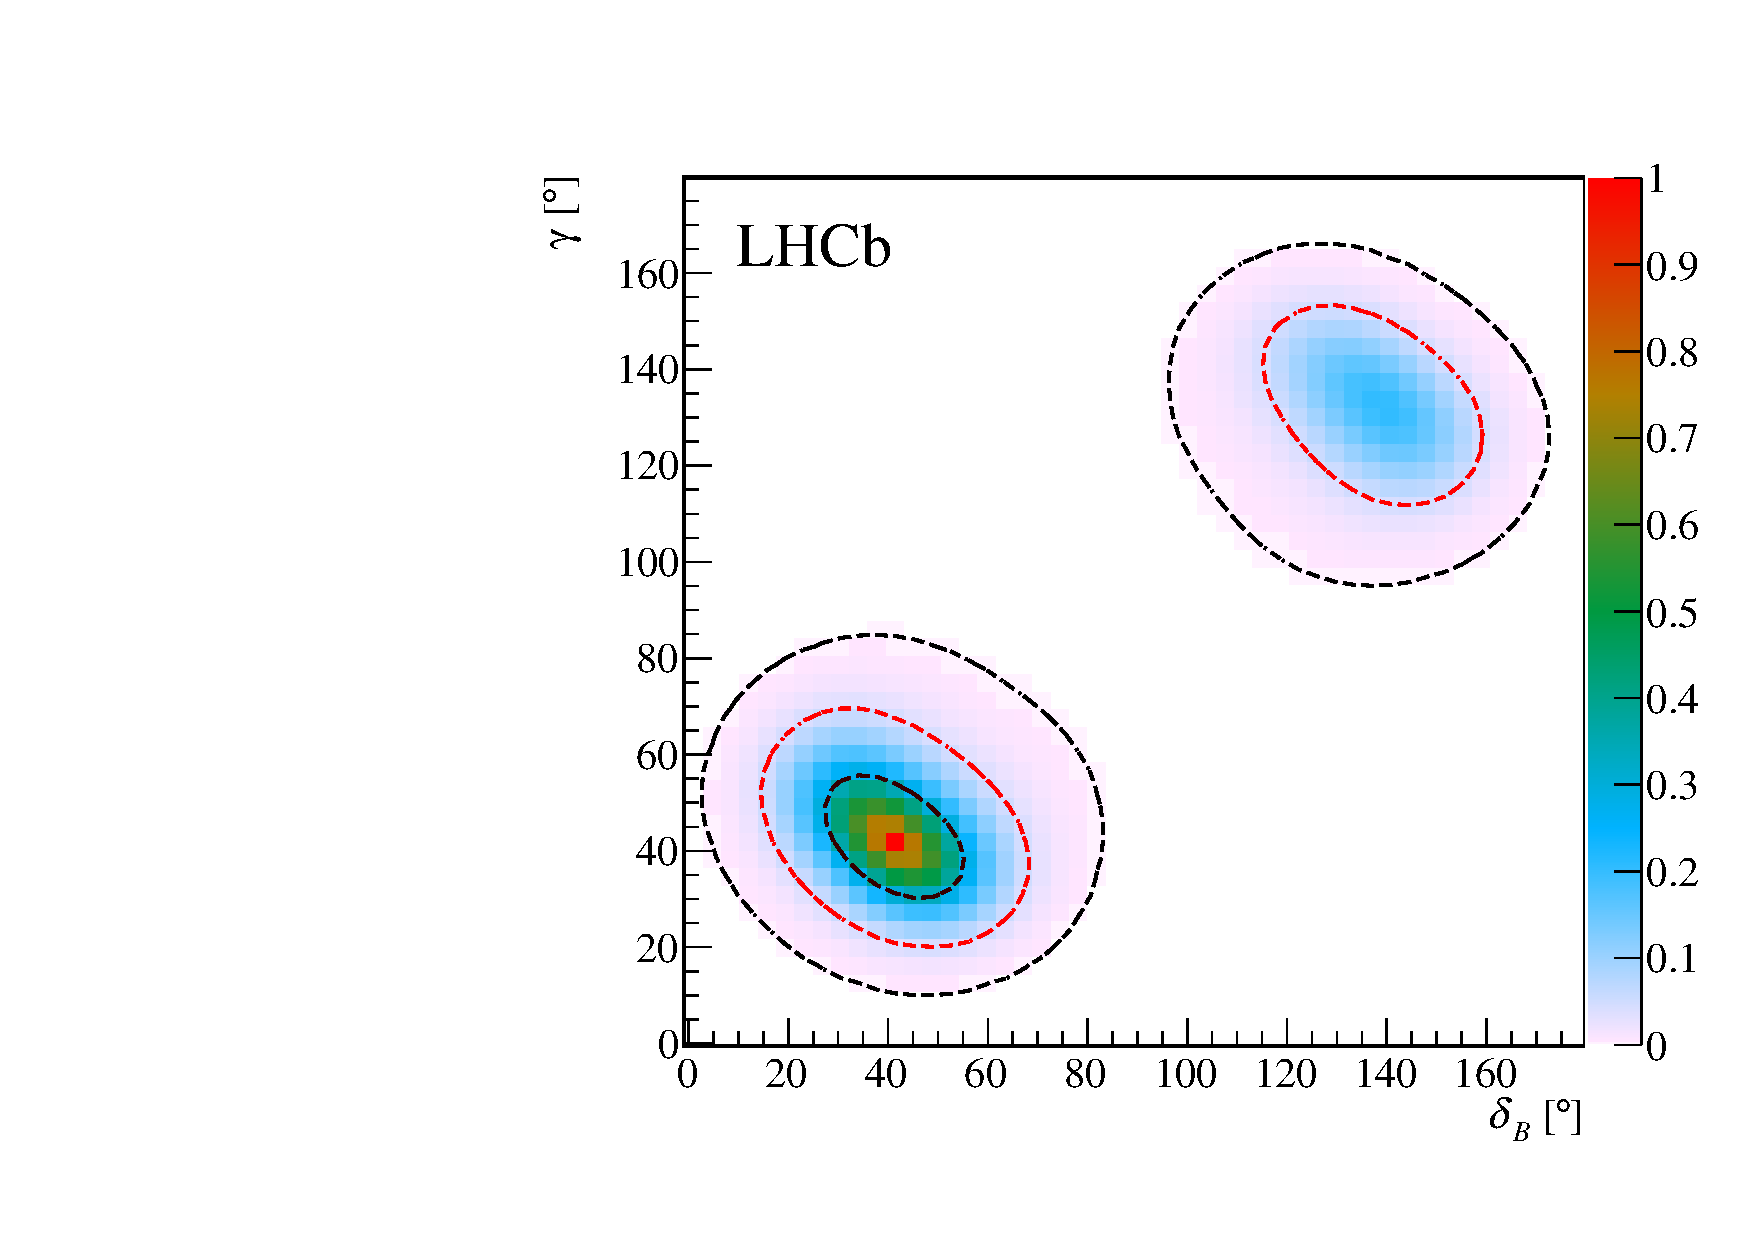
\includegraphics[width=0.5\linewidth]{figures/interpretation/deltaBu_dkstar_gamma_2Dscan_nomixing_Run2.pdf}}
\caption{Contour plots showing projected 2D scans of the physics parameters at the end of \runtwo, assuming the central values remain the same. The dashed lines represent the $\Delta \chi^2 = 2.30,\ 6.18,\ 11.8$ contours, corresponding to 68.3\%, 95.5\%, 99.7\% confidence levels (CL), respectively. The colour scale represents 1 - CL.}
\label{gammadiniplotsrun2}
\end{figure}

\begin{figure}[h]
\centering
\subfloat[\rb versus \Pgamma]{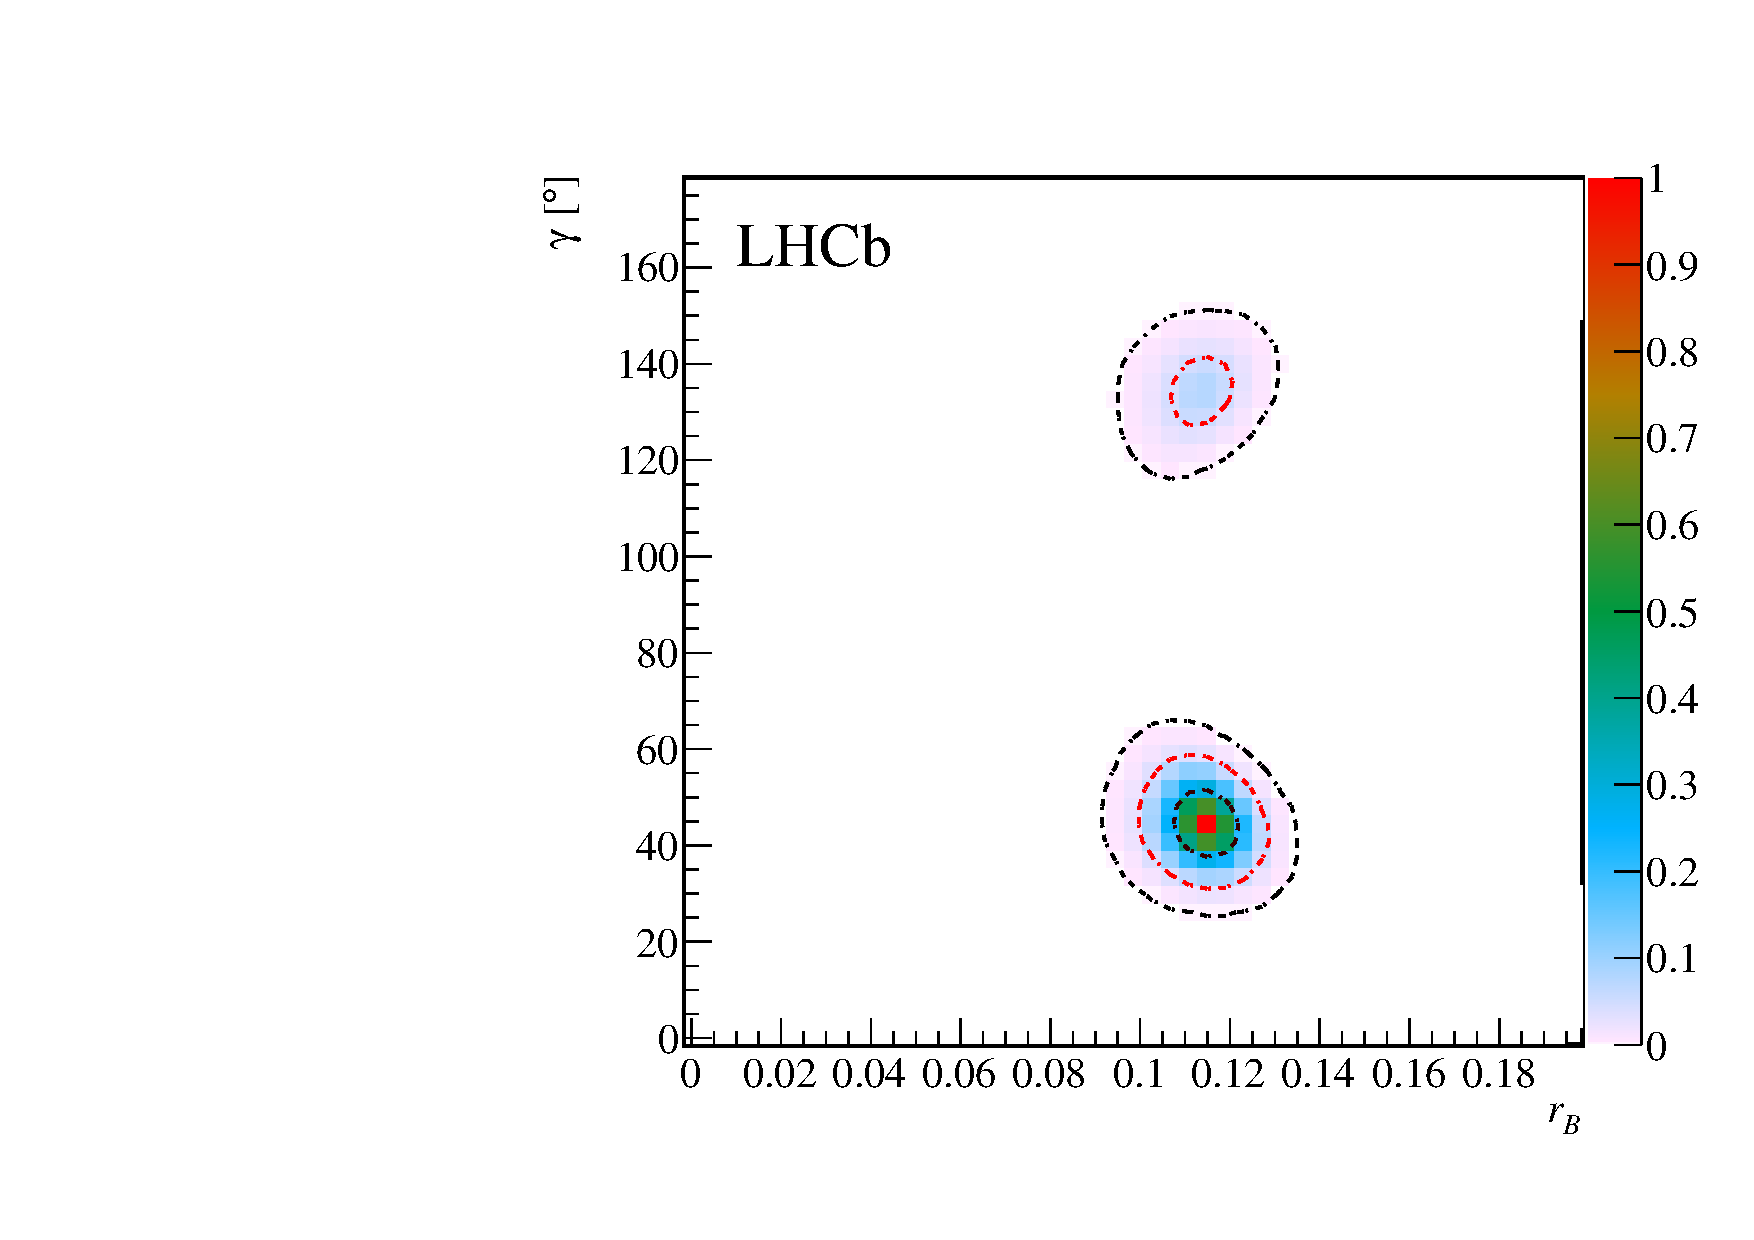
\includegraphics[width=0.5\linewidth]{figures/interpretation/rBu_dkstar_gamma_2Dscan_nomixing_Run3.pdf}}
\subfloat[\deltab versus \Pgamma]{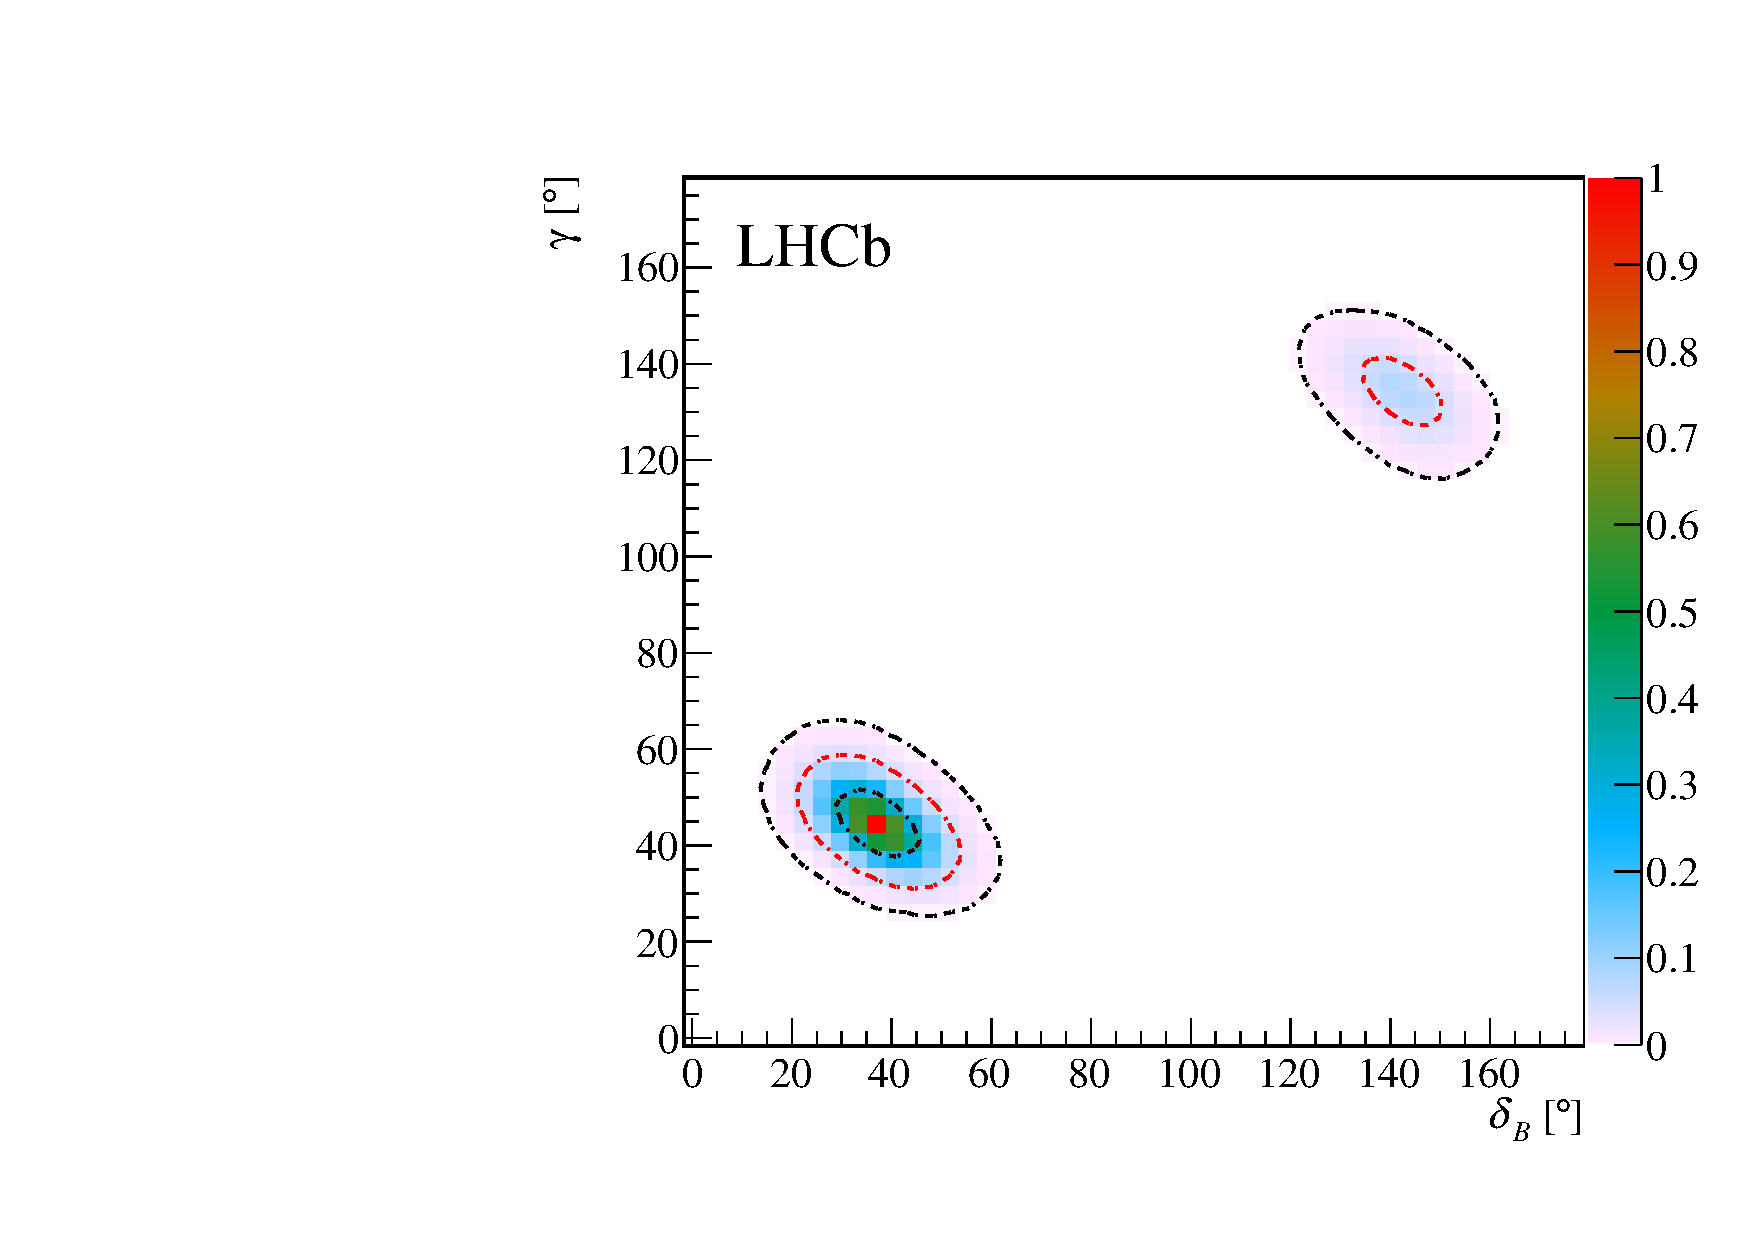
\includegraphics[width=0.5\linewidth]{figures/interpretation/deltaBu_dkstar_gamma_2Dscan_nomixing_Run3.pdf}}
\caption{Contour plots showing projected 2D scans of the physics parameters at the end of Run 3, assuming the central values remain the same. The dashed lines represent the $\Delta \chi^2 = 2.30,\ 6.18,\ 11.8$ contours, corresponding to 68.3\%, 95.5\%, 99.7\% confidence levels (CL), respectively. The colour scale represents 1 - CL.}
\label{gammadiniplotsrun3}
\end{figure}

It can be seen that the sensitivity continues to improve with more data, as the uncertainties are dominated by statistical uncertainty, therefore this channel will continue to benefit from the increased dataset in Run 3 and beyond. At the end of Run 3 the uncertainty on \Pgamma, from \btodkst decays investigated in this thesis, is expected to reduce to about $5^{\circ}$. Uncertainties in the measurements of the hadronic parameters in \btodkst decays, \rb and \deltab, will also reduce significantly to about $0.006$ and $7^{\circ}$ respectively. However, it can be observed from Figure \ref{gammadiniplotsrun3} that even with this additional data, multiple solutions still remain. This problem of multiple solutions can be resolved by investigating alternative decays of the \Dz meson via a different method, referred to as the GGSZ method after the theorists Giri, Grossman, Soffer and Zupan~\cite{GGSZ}, which involves analysing \D decays to \KS\pip\pim and \KS\Kp\Km final states~\cite{LHCb-PAPER-2012-027,LHCb-PAPER-2014-041}.

The field of \Pgamma measurements is dominated, and will continue to be dominated, by \decay{\Bm}{\D\Km} measurements. However, the analysis of this decay mode requires modeling several problematic backgrounds, most noteably the misidetification background from \decay{\Bm}{\D\pim} decays and the partially reconstructed background, which both overlap with the signal region. Therefore, all \decay{\Bm}{\D\pim} measurements are accompanied by systematic uncertainties relating to these backgrounds. Expanding the field of \Pgamma-senstive measurements to include other \Bm decays, namely \decay{\Bm}{\D\Kstarm} decays, which contains relatively few problematic background components, provides a cross-check for the \Pgamma measurements made with \decay{\Bm}{\D\pim} decays.

Additionally, this thesis has presented the current best sensitivity to the hadronic parameters of the \Bm decay, namely \rb and \deltab. Further studies into \btodkst decays would lead to the development of an amplitude model for \decay{\Bm}{\D\KS\pim} decays to gain a greater understanding of resonant structures present in the \KS\pim system. This investigation would require the parameters \rb and \deltab as constraints in the model, which can only be provided by studies of \btodkst decay as presented in this thesis. 

When combining \Pgamma measurements, the \decay{\Bm}{\D\Km} channel is the most widely used and most sensitive to \Pgamma~\cite{LHCb-PAPER-2016-032}. Different methods have been developed to investigate a range of decays modes of the \Dz meson using the \decay{\Bm}{\D\Km} channel. The work presented in this thesis leads the way for a completely new, physically similar \decay{\Bm}{\D\Kstarm} channel to be exploited using the many different \D decay modes developed for the \decay{\Bm}{\D\Km} channel. This work opens the door to a whole new range of \Pgamma-sensitive analyses to be developed. The work in this thesis can be further expanded by considering \decay{\Bm}{\D\Kstarm} decays, where the \Kstarm meson is reocnstructed as \Km\piz. The inclusion of this alternative mode would results in a gain in \Pgamma-senstivity from the additional data. However, as mentioned previously, theis mode is significantly more difficult to reconstruct and is not included in this thesis as it would not provide significant additional sensitivity with the current dataset.

The expected sensitivity to \Pgamma at the end of Run 2 is $4^{\circ}$~\cite{LHCb-PAPER-2012-031}. The upgrade after Run 2 is estimated to provide a luminosity of 50\invfb by the end of 2030, and achieve a significant increase in signal efficiency for \B meson decays, resulting in a predicted sensitivity to \Pgamma of $0.9^{\circ}$ by the end of 2030~\cite{LHCb-PAPER-2012-031}. The Belle II experiment, which is expecting to collect a data sample corresponding to an integrated luminosity of 50$ab^{\text{-1}}$ between 2018 and 2026, predicts a determination of \Pgamma to $1.6^{\circ}$~\cite{BelleII}.

\clearpage
